\documentclass[12pt,twoside,openright]{book}
\usepackage[utf8]{inputenc}
\usepackage[T1]{fontenc}
\usepackage[spanish,es-noquoting]{babel}

% Standard Amazon KDP Hardcover size: 5.5 x 8.5 inches (139.7 x 215.9 mm)
\usepackage[paperwidth=5.5in, paperheight=8.5in, top=24mm, bottom=24mm, inner=24mm, outer=20mm, footskip=12mm]{geometry}

\usepackage{titlesec}
\usepackage{fancyhdr}
\usepackage{setspace} % For line spacing
\usepackage{graphicx}
\graphicspath{ {images/} }
\usepackage{needspace}
\usepackage{microtype}
\usepackage{csquotes}
\usepackage[scaled=1.11]{ebgaramond} % Professional Garamond font
\usepackage[parfill]{parskip} % Spacing between paragraphs
\usepackage{xcolor}
\usepackage{qrcode} % For generating QR codes directly in PDF
\usepackage[export]{adjustbox} % For image borders
\usepackage[framemethod=TikZ]{mdframed} % For elegant frames around text
\usepackage{emptypage} % Clears headers and footers on empty right-hand separator pages

% Line spacing - airy and comfortable for Hardcover
\setstretch{1.45}

\usepackage{caption}
\captionsetup[figure]{font={small,it}, labelformat=empty, skip=6pt, justification=centering}

% Section styling - elegant Garamond headers
\titleformat{\chapter}[display]
  {\normalfont\Huge\bfseries\itshape\centering}{\chaptertitlename\ \thechapter}{6pt}{\Huge}
\titlespacing*{\chapter}{0pt}{15pt}{30pt}

\setlength{\headheight}{16pt}

% Header/Footer
\pagestyle{fancy}
\fancyhf{}
\fancyhead[LE,RO]{\small\thepage}
\fancyhead[RE]{\small\itshape\nouppercase{Mi amigo Jesucristo}}
\fancyhead[LO]{\small\itshape\nouppercase{\leftmark}}
\renewcommand{\headrulewidth}{0.4pt}

% Fix for long titles in headers
\renewcommand{\chaptermark}[1]{\markboth{#1}{}}

\usepackage{url}
\usepackage{hyperref}
\begin{document}

\frontmatter

% Portadilla (Half-Title)
\thispagestyle{empty}
\vspace*{5cm}
\begin{center}
    {\LARGE \textbf{Mi amigo Jesucristo}}
\end{center}
\cleardoublepage

% Portada Principal (Full Title Page)
\begin{titlepage}
    \centering
    \vspace*{2cm}
    {\Huge \textbf{Mi amigo Jesucristo} \par}
    \vspace{0.8cm}
    {\Large \textit{Una guía cuántica para el alma moderna} \par}
    \vfill
    {\large \textbf{A Glimpse of Light} \par}
    \vspace{0.5cm}
    {\small Con arte y música de Maria Paz Arés Osset \par}
    \vspace*{2cm}
\end{titlepage}
\cleardoublepage

% Copyright Page
\thispagestyle{empty}
\vspace*{11cm}
\begin{center}
    \small
    \textbf{Mi amigo Jesucristo} \\
    \textit{Una guía cuántica para el alma moderna} \\
    \vspace{0.5cm}
    © 2024 A Glimpse of Light \\
    Todos los derechos reservados. \\
    Publicado en Amazon KDP (Edición Tapa Dura) \\
    \vspace{0.3cm}
    \textit{www.pazaresosset.es}
\end{center}
\cleardoublepage

% Epigraph / Cita inspiradora
\thispagestyle{empty}
\vspace*{6cm}
\begin{center}
    \itshape
    «El Reino de los Cielos no es un lugar al que se llega,\\
    es una frecuencia que se sintoniza.»\\
    \vspace{1cm}
    \normalfont --- \textbf{Mi Amigo Jesucristo}
\end{center}
\cleardoublepage

\tableofcontents
\cleardoublepage

\mainmatter

\chapter*{Introducción: Entre la Partícula y la Vibración}
\addcontentsline{toc}{chapter}{Introducción: Entre la Partícula y la Vibración}
\markboth{Introducción: Entre la Partícula y la Vibración}{Introducción: Entre la Partícula y la Vibración}
\vspace{0.6cm}
\begin{center}
\nopagebreak
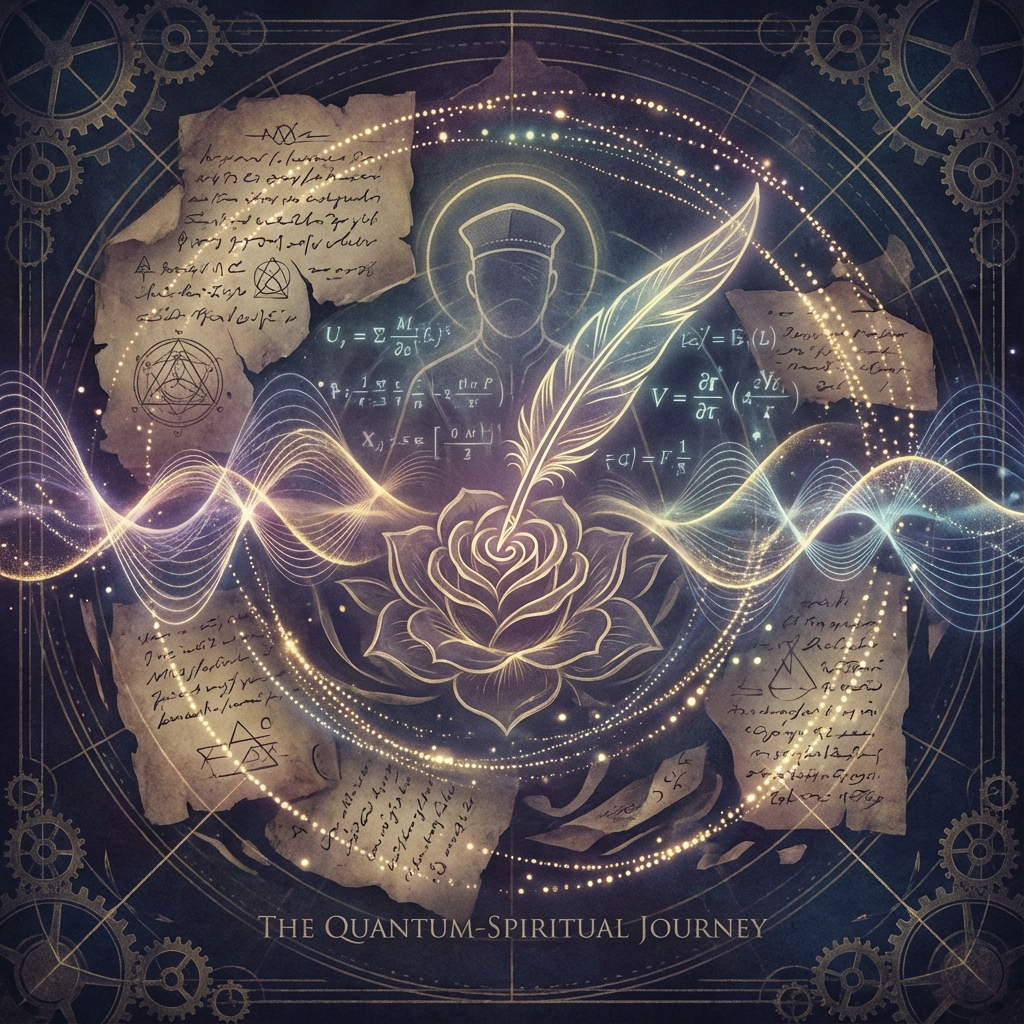
\includegraphics[width=0.75\textwidth,cfbox=gray!60 0.6pt 4pt]{intro_quantum_luther.png}\\
\vspace{4pt}
{\small\itshape Entre la partícula y la vibración: el despertar de la conciencia.}
\end{center}

\vspace{0.6cm}
\section*{I. La Inquietud del Alma}

Desde que tengo uso de razón, he sentido una especie de vibración disonante cuando me acercaba a los grandes templos de piedra. No era falta de fe; al contrario, siempre he intuido que detrás del velo de la realidad existe una Fuente inagotable de amor. Mi conflicto, mi tormento silencioso, nacía del contraste entre esa intuición de un Dios infinito y la pequeñez de las cajas en las que intentábamos meterlo.

Crecí en el seno del catolicismo, respirando el incienso y admirando la liturgia, pero muy pronto, esa belleza se vio empañada por una sensación incómoda: la soberbia. Me dolía en el alma escuchar, implícita o explícitamente, que nosotros teníamos «la verdad» y los demás no. ¿Cómo podía ser que el Creador de un universo de cien mil millones de galaxias tuviera preferencia por un código postal espiritual concreto? Sentía que pecábamos de una arrogancia terrible al no reconocer la salvación para otros credos, al mirar con lástima o superioridad a quien buscaba la luz por otro camino. Esa exclusividad me parecía, paradójicamente, el acto más irreligioso de todos: limitar la misericordia de Dios a nuestras propias fronteras humanas.

\section*{II. Las Sombras en los Centros de Poder}

Pero mi tormento iba más allá de la teología. Al estudiar la historia, me topaba con muros manchados de sangre. La Inquisición, las cruzadas, las excomuniones... No podía evitar pensar: ¿Cómo hemos llegado de «ama a tu prójimo» a «quémalo si no piensa como tú»?

Durante años, esto me alejó. Sentía rabia. Veía la institución y solo veía las sombras. Sin embargo, con el tiempo y la madurez, entendí algo fundamental: la Iglesia, como cualquier estructura humana, está compuesta de personas. Y las personas somos antenas. Cuando el miedo se instala en los centros de poder, cuando la necesidad de control supera a la necesidad de servir, la vibración colectiva desciende.

La Inquisición no fue obra de Dios, ni siquiera fue obra de «la religión» en abstracto. Fue la consecuencia inevitable de una \textbf{baja vibración} instalada en la cúpula. El miedo a perder el poder, el miedo a lo diferente, el odio disfrazado de celo... todo eso son frecuencias densas, pesadas. Y cuando esa densidad se apodera de una jerarquía, el resultado es el sufrimiento. Obviamente, es algo que el propio Cristo, mi amigo Jesús, jamás hubiera permitido. Él, que detuvo las piedras contra la adúltera, jamás hubiera encendido una hoguera.

Entender esto me permitió perdonar. Entendí que no era «la Iglesia» la que fallaba, sino la vibración de los hombres que, en momentos oscuros, la dirigían. Y que, por debajo de esa cúpula de poder, siempre hubo miles de curas, monjas y laicos vibrando alto, dando de comer al hambriento, consolando al triste, manteniendo encendida la luz a pesar de la oscuridad de sus líderes.

\section*{III. La Física Cuántica del Espíritu}

Mi reconciliación definitiva llegó de la mano de la ciencia. Siempre me ha fascinado la física cuántica, esa rama del saber que nos dice que la realidad no es tan sólida como parece. Nos enseña que toda partícula subatómica es, a la vez, materia y onda. Es algo concreto y, al mismo tiempo, es pura vibración, pura posibilidad.

Ahí fue donde todo hizo clic. El Padre Nuestro, las enseñanzas de Jesús... no eran normas morales rígidas, ¡eran instrucciones de física cuántica!

Cuando Jesús nos dice «no temáis», no nos está dando una orden psicológica, nos está diciendo: «No bajéis vuestra frecuencia». El miedo es una vibración lenta, densa, que contrae la realidad. El amor, la paz, la seguridad... son vibraciones rápidas, expansivas, que crean luz.

Entendí que «caer en la tentación» no es comerse un pastel en cuaresma. Es la tentación de dejarse arrastrar por la gravedad de las bajas vibraciones: el odio, la venganza, la envidia, la soberbia. Cuando odias, te densificas. Te conviertes en «partícula» pesada, aislada, desconectada del todo. Cuando amas, te conviertes en «onda», te expandes, te conectas con el campo cuántico universal, con el Padre.

\section*{IV. Un Café con Lutero}

En este viaje de comprensión, a menudo me he imaginado tomando un café con Martín Lutero en el siglo XVI. Creo que habríamos sido buenos amigos. Él vio esa misma soberbia que a mí me atormentaba. Vio cómo la estructura se había vuelto tan densa, tan preocupada por vender bulas y construir basílicas de mármol, que se había olvidado de la vibración del Evangelio.

Lutero tuvo la valentía de decir: «La salvación no está en Roma, está en tu fe». Y yo añadiría, desde mi perspectiva del siglo XXI: «La salvación no depende de seguir al Papa, sino de la frecuencia de tu corazón».

Si tus obras, si tu vida diaria, están hechas desde la alta vibración del amor, no cabe duda de que estás salvado. Porque «estar salvado» no es un ticket para entrar en un club VIP después de morir. Estar salvado es vivir, aquí y ahora, en la frecuencia del Paraíso. Es estar en sintonía con la Fuente.

Si un budista, un ateo o un cristiano vibran en el amor incondicional, están en la misma frecuencia. Están «en Dios». Y ninguna bula, ningún decreto, puede cambiar esa realidad física y espiritual. La salvación es una cuestión de resonancia, no de burocracia.

\section*{V. La Luz que Prevalece}

Por eso escribo este libro. No para atacar a la religión, sino para rescatar su esencia vibracional. Escribo desde el amor, habiendo sanado esa lástima que sentía por la soberbia institucional. He dejado de mirar la oscuridad de la Inquisición para mirar la luz de los místicos, de los santos anónimos, de la gente buena que, en nombre de esa misma fe, ha vibrado tan alto que ha cambiado el mundo.

Este libro es una invitación a caminar con Jesús, no como un juez severo, sino como un maestro de vibración. Un amigo que nos enseña a navegar entre Madrid, Las Rozas y Colmenarejo sin perder la sintonía. Un guía que nos recuerda, una y otra vez, que somos luz, que somos onda, y que nuestro único deber es mantener la frecuencia alta, pase lo que pase a nuestro alrededor.

Así que, querido lector, olvida por un momento los dogmas, las culpas y los miedos heredados. Abre tu mente a la posibilidad de que todo, absolutamente todo, es música. Y que tú tienes el instrumento en tus manos para tocar la melodía más hermosa.

Bienvenido a «Mi amigo Jesucristo».
\cleardoublepage

\chapter{El Encuentro en Madrid}
\vspace{0.6cm}
\begin{center}
\nopagebreak
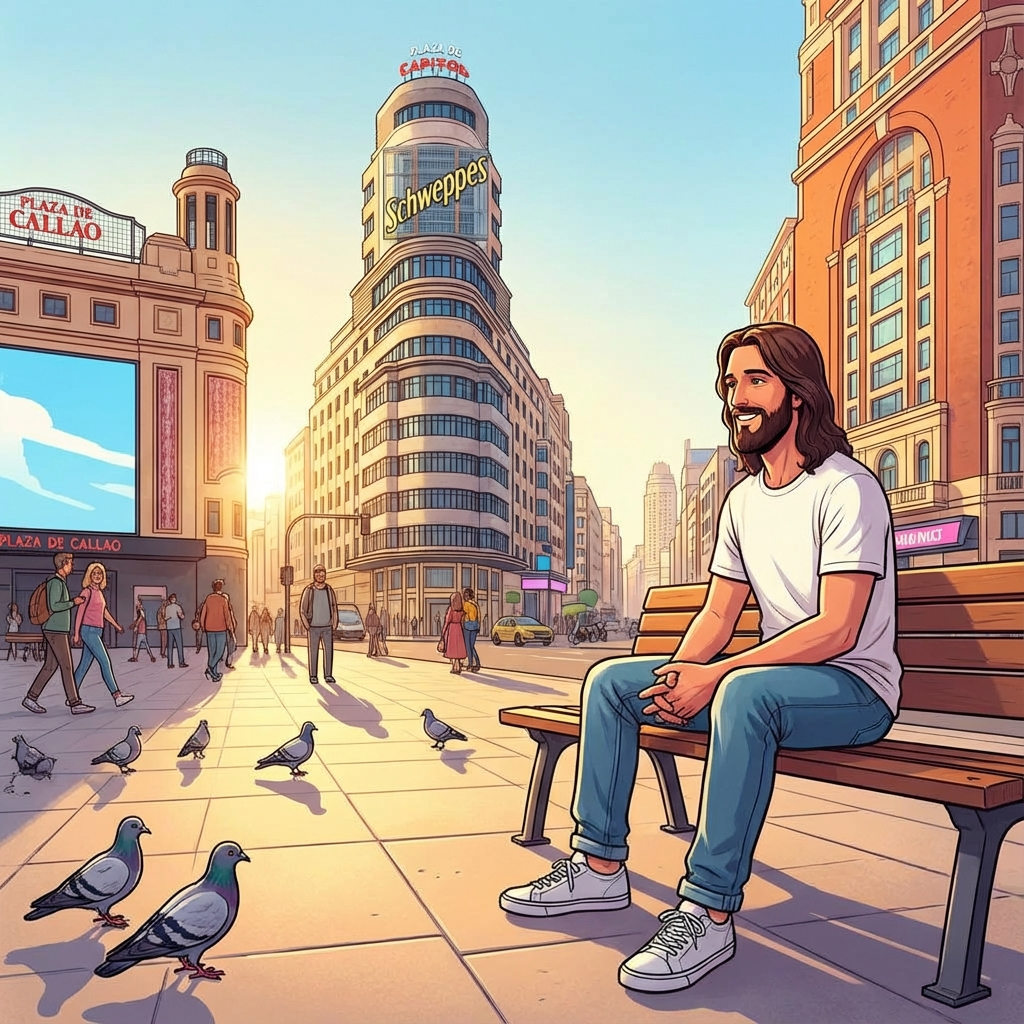
\includegraphics[width=0.75\textwidth,cfbox=gray!60 0.6pt 4pt]{madrid.png}\\
\vspace{4pt}
{\small\itshape El encuentro en la ciudad: la presencia viva en lo cotidiano.}
\end{center}

\vspace{0.6cm}
Era una tarde de primavera en Madrid. El sol se filtraba entre los edificios de la Gran Vía, creando juegos de luces y sombras que parecían danzar sobre el asfalto. Yo caminaba con la prisa habitual de quien vive en la ciudad, con la mente llena de ruido: correos por responder, facturas, preocupaciones... vibrando bajo, muy bajo.

De repente, en la plaza de Callao, lo vi. No llevaba túnica, ni sandalias, ni tenía un halo brillante sobre la cabeza. Llevaba unos vaqueros desgastados, una camiseta blanca y unas zapatillas cómodas. Estaba sentado en un banco, mirando a la gente pasar con una sonrisa tranquila, una sonrisa que parecía detener el tiempo.

—Hola, Francisco —dijo cuando pasé cerca.

Me detuve en seco. Nadie me llamaba por mi nombre completo en la calle, y menos un desconocido. Pero al mirarlo a los ojos, supe que no era un desconocido. Había una familiaridad ancestral en su mirada, una paz que desarmaba cualquier defensa.

—¿Jesús? —pregunté, sintiéndome un poco ridículo.

—El mismo —respondió él, dándome una palmada en el espacio vacío del banco a su lado—. Siéntate un rato. Estás vibrando en una frecuencia que me está dando dolor de cabeza, y eso que yo aguanto mucho.

Me senté, todavía aturdido.
—¿Vibrando? —repetí.

—Sí, vibrando. Todo es vibración, amigo mío. El miedo, la prisa, el enfado... son vibraciones densas, pesadas. Te anclan al suelo y no te dejan ver el cielo, aunque lo tengas encima.

Miré hacia arriba. El cielo de Madrid estaba de un azul intenso, precioso. No me había fijado hasta ese momento.

—He venido a pasar unos días contigo —continuó—. Vamos a dar una vuelta. Necesitas recordar cómo sintonizar la radio de tu alma. Estás escuchando pura estática.

Y así, en medio del bullicio de Madrid, comenzó la aventura más extraña y maravillosa de mi vida. No con milagros de convertir agua en vino, sino con el milagro de transformar mi ruido interno en música.
\cleardoublepage

\chapter{Paseo por Las Rozas}
\vspace{0.6cm}
\begin{center}
\nopagebreak
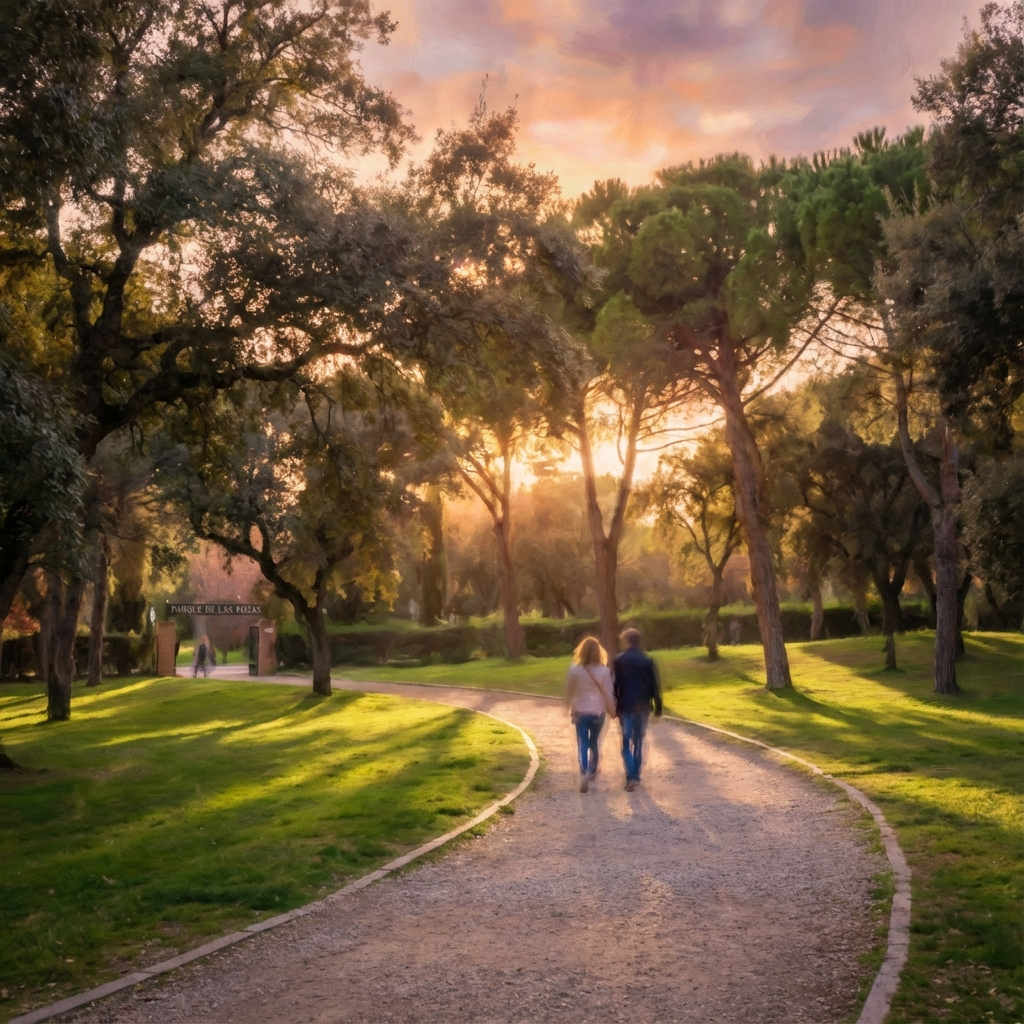
\includegraphics[width=0.75\textwidth,cfbox=gray!60 0.6pt 4pt]{las_rozas_park.png}\\
\vspace{4pt}
{\small\itshape El silencio del parque: afinando el templo interior.}
\end{center}

\vspace{0.6cm}
Al día siguiente, decidimos alejarnos un poco del centro. Fuimos a Las Rozas. Jesús quería ver cómo vivía la gente en las afueras, en esas urbanizaciones donde parece que todo está ordenado pero donde a veces el caos se esconde detrás de las puertas blindadas.

Caminábamos por el parque París. Él se detenía a oler las flores, a tocar la corteza de los árboles.
—¿Ves esto? —me dijo, señalando un roble—. Él no se preocupa por si mañana lloverá o si hará sol. Simplemente es. Está en su centro. Vibra en la frecuencia de la vida.

—Es fácil para un árbol —repliqué—. No tiene hipoteca.

Jesús se rió a carcajadas. Una risa limpia, contagiosa.
—La hipoteca... el gran monstruo moderno. Mira, Francisco, el problema no es la deuda del banco. El problema es la deuda que crees tener con el futuro. Vives pagando por adelantado con tu ansiedad un tiempo que aún no existe.

Nos sentamos en el césped. Un perro vino corriendo y le lamió la mano. Él lo acarició con ternura.
—«Danos hoy nuestro pan de cada día» —murmuró—. La gente cree que hablo solo de comida. Hablo de la energía necesaria para el \textit{ahora}. Cuando te preocupas por el mes que viene, estás gastando la energía de hoy en un problema imaginario. Bajas tu vibración. Te debilitas.

—¿Y cómo se sube la vibración? —pregunté, sintiendo que empezaba a entender.

—Agradeciendo —dijo él, mirando el lago artificial—. El agradecimiento es el ascensor del alma. Si agradeces este sol, este aire, este momento... subes. Si te quejas de lo que te falta... bajas. Es física espiritual básica.

En Las Rozas, entre chalets y coches de alta gama, aprendí que la verdadera riqueza no estaba en lo que poseíamos, sino en la capacidad de disfrutar lo que ya estaba ahí, gratis, para todos.
\cleardoublepage

\chapter{La Vibración y el Silencio}
\vspace{0.6cm}
\begin{center}
\nopagebreak

\includegraphics[width=0.75\textwidth,cfbox=gray!60 0.6pt 4pt]{silence_vibration.png}\\
\vspace{4pt}
{\small\itshape La vibración del silencio: trascendiendo el ruido mental.}
\end{center}

\vspace{0.6cm}
Tomamos el autobús hacia la sierra. El paisaje iba cambiando, volviéndose más verde, más salvaje. Jesús miraba por la ventana como un niño en su primera excursión.

—El ruido —dijo de repente—. Es la gran enfermedad de este siglo. No el ruido de los coches, sino el ruido de las pantallas, de las notificaciones, de las opiniones constantes.

Llegamos a un punto intermedio antes de Colmenarejo. Nos bajamos en un camino de tierra.
—Vamos a practicar el silencio —propuso.

—¿Callarnos?

—No solo callar la boca. Callar la mente. Quiero que escuches la vibración del universo.

Caminamos en silencio durante una hora. Al principio, mi mente era una lavadora centrifugando pensamientos: «¿Qué hago aquí caminando con Jesucristo?», «¿Me habré vuelto loco?», «Tengo que llamar a mi madre...». Pero poco a poco, el ritmo de mis pasos y la respiración tranquila de mi acompañante me fueron calmando.

Nos detuvimos en un alto desde donde se veía el horizonte.
—Cierra los ojos —me susurró—. Siente.

Lo hice. Y por primera vez en mucho tiempo, no sentí miedo. Sentí una especie de zumbido suave, cálido. Como si el aire me abrazara.

—Eso es —dijo él, como si pudiera leer mi sensación—. Eso es vibrar alto. Es la frecuencia del Amor. No el amor romántico de las películas, sino el Amor que sostiene los átomos unidos. Cuando estás ahí, nada puede tocarte. «Líbranos del mal» no es pedir que no existan los malos. Es pedir estar en una frecuencia donde la maldad no te alcance, donde no resuene contigo.

Abrí los ojos. El mundo parecía más brillante.
—Si vibras alto, el bajo no te ve —concluyó—. Es como si fueras invisible para la oscuridad.
\cleardoublepage

\chapter{Colmenarejo y la Naturaleza}
\vspace{0.6cm}
\begin{center}
\nopagebreak
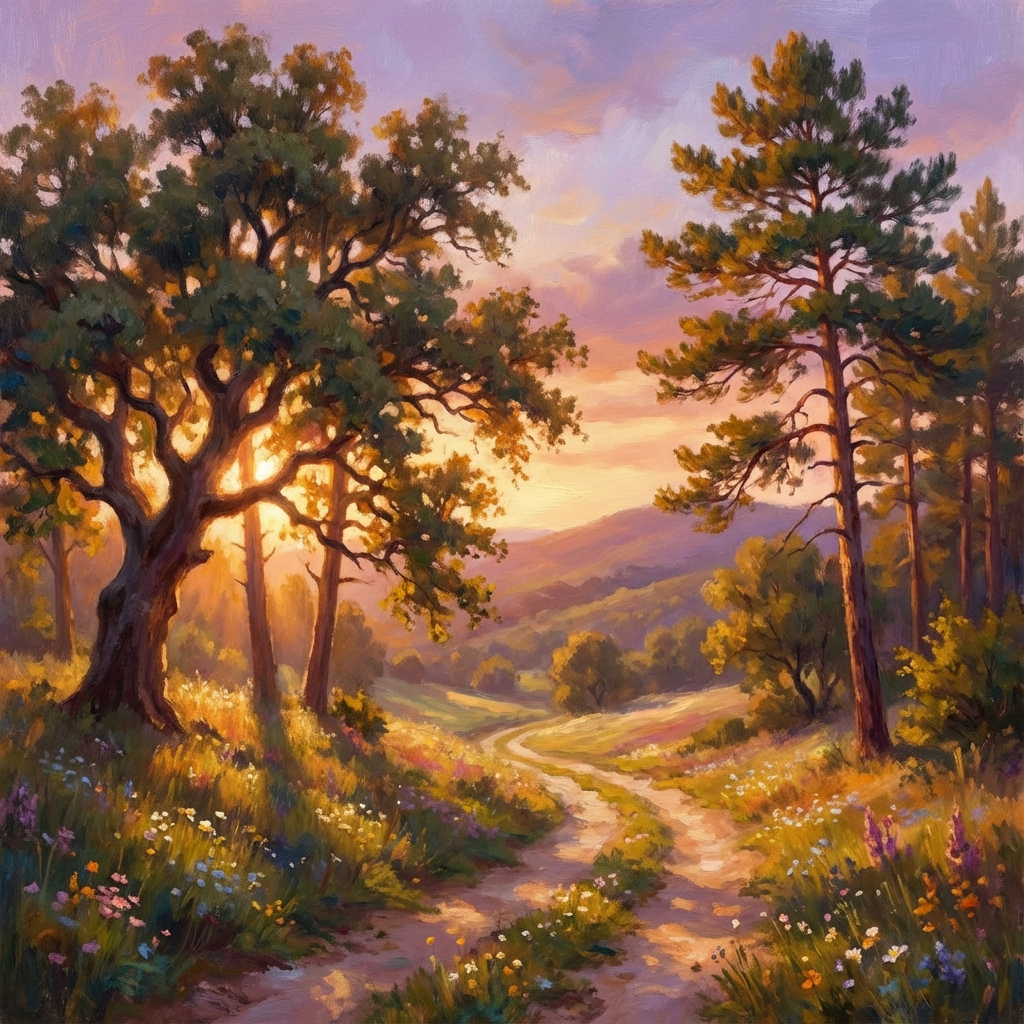
\includegraphics[width=0.75\textwidth,cfbox=gray!60 0.6pt 4pt]{nature.png}\\
\vspace{4pt}
{\small\itshape La rendición y la paz: el flujo natural del Ser.}
\end{center}

\vspace{0.6cm}
Llegamos a Colmenarejo al atardecer. El pueblo tenía ese encanto de lo que está a medio camino entre la urbe y el campo. Fuimos hacia la zona de la Universidad, donde hay grandes espacios abiertos y se respira otro aire.

—Aquí se siente mejor —dijo Jesús, inspirando profundamente—. La naturaleza es la gran maestra de la vibración. Ella nunca se equivoca. Un pino no intenta ser una encina. Un río no intenta fluir hacia arriba.

Nos sentamos cerca de la ermita. El cielo se teñía de naranjas y violetas.
—Padre Nuestro que estás en los cielos... —empezó a recitar suavemente—. ¿Sabes dónde está el cielo, Francisco?

—¿Arriba? —señalé.

Él negó con la cabeza sonriendo.
—El cielo es un estado de conciencia. Es ese lugar interno donde todo está bien, donde hay paz absoluta. «Que estás en los cielos» significa que la Fuente de todo reside en esa alta vibración. Y tú tienes un acceso directo ahí. Tienes wifi directo con el Creador, pero a veces se te olvida la contraseña.

—¿Cuál es la contraseña?

—La rendición. Dejar de luchar contra lo que es. Aceptar. Fluir. Cuando te rindes a la vida, dejas de nadar contracorriente. Y entonces, la corriente te lleva. Y la corriente de la vida siempre te lleva hacia el bien, hacia el mar.

En Colmenarejo, bajo las primeras estrellas, entendí que rezar no era pedir cosas como quien hace la lista de la compra. Rezar era sintonizar. Era volver a poner el dial en la frecuencia correcta para escuchar la música que siempre está sonando, aunque nosotros estemos demasiado ocupados haciendo ruido para oírla.
\cleardoublepage

\chapter{El Padre Nuestro (Parte 1: Padre)}
\vspace{0.6cm}
\begin{center}
\nopagebreak
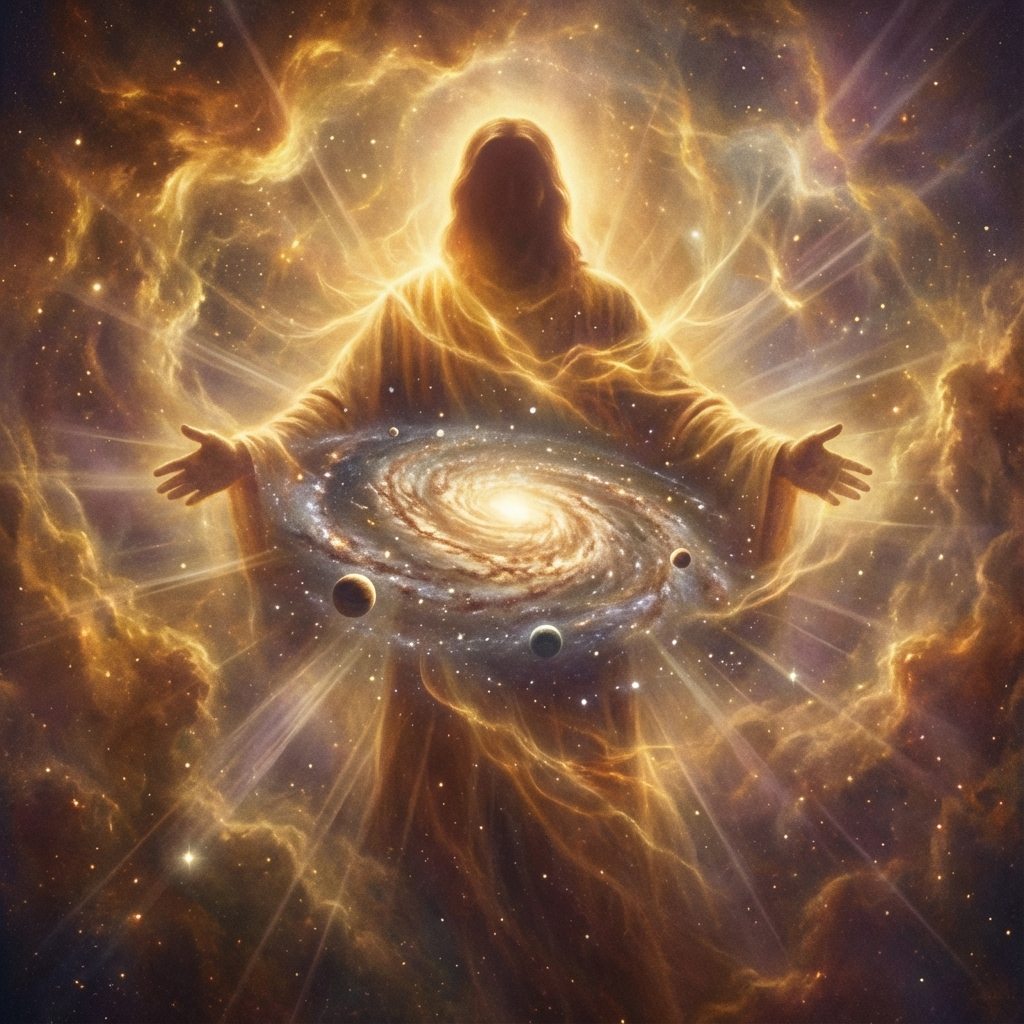
\includegraphics[width=0.75\textwidth,cfbox=gray!60 0.6pt 4pt]{cosmic_father.png}\\
\vspace{4pt}
{\small\itshape Abwoon: la Fuente cósmica de toda la creación.}
\end{center}

\vspace{0.6cm}
Regresamos a Madrid, pero esta vez fuimos al Retiro. Nos sentamos cerca del Palacio de Cristal.
—Hablemos de tu padre —dijo Jesús de repente.

Me tensé. Mi relación con mi padre no siempre había sido fácil.
—¿Por qué?

—Porque la oración empieza con «Padre Nuestro». Y mucha gente se atasca ahí. Si tu padre terrenal fue duro, o ausente, o crítico, proyectas esa imagen en Dios. Crees que Dios es un señor con barba que te vigila para castigarte si te equivocas.

Cogió una piedra del suelo y la lanzó al estanque. Las ondas se expandieron.
—La palabra «Padre» en arameo, \textit{Abwoon}, tiene un significado mucho más amplio. Es la Fuente, el Origen, la Respiración de la Vida. No es un señor. Es una Energía. Es la vibración original de la que todos salimos.

—Entonces, ¿no es un juez?

—¡Claro que no! —exclamó—. ¿Juzga el sol a las flores? ¿Les dice «tú sí floreces, te doy luz; tú no, te quedas a oscuras»? El sol brilla para todas. Dios es Amor incondicional. Si tú te cierras en una cueva, no es culpa del sol que estés a oscuras. Es tu elección.

—¿Y por qué «Nuestro»?

—Porque no es «Mío». No es propiedad privada de ninguna religión, ni de ninguna persona. Es de todos. Del cristiano, del budista, del ateo, del árbol y del perro. Todos venimos de la misma Fuente. Reconocer eso es el primer paso para vibrar alto: la Unidad. Si te ves separado de los demás, bajas tu vibración. Si te ves unido, subes.
\cleardoublepage

\chapter{El Padre Nuestro (Parte 2: Cielo)}
\vspace{0.6cm}
\begin{center}
\nopagebreak
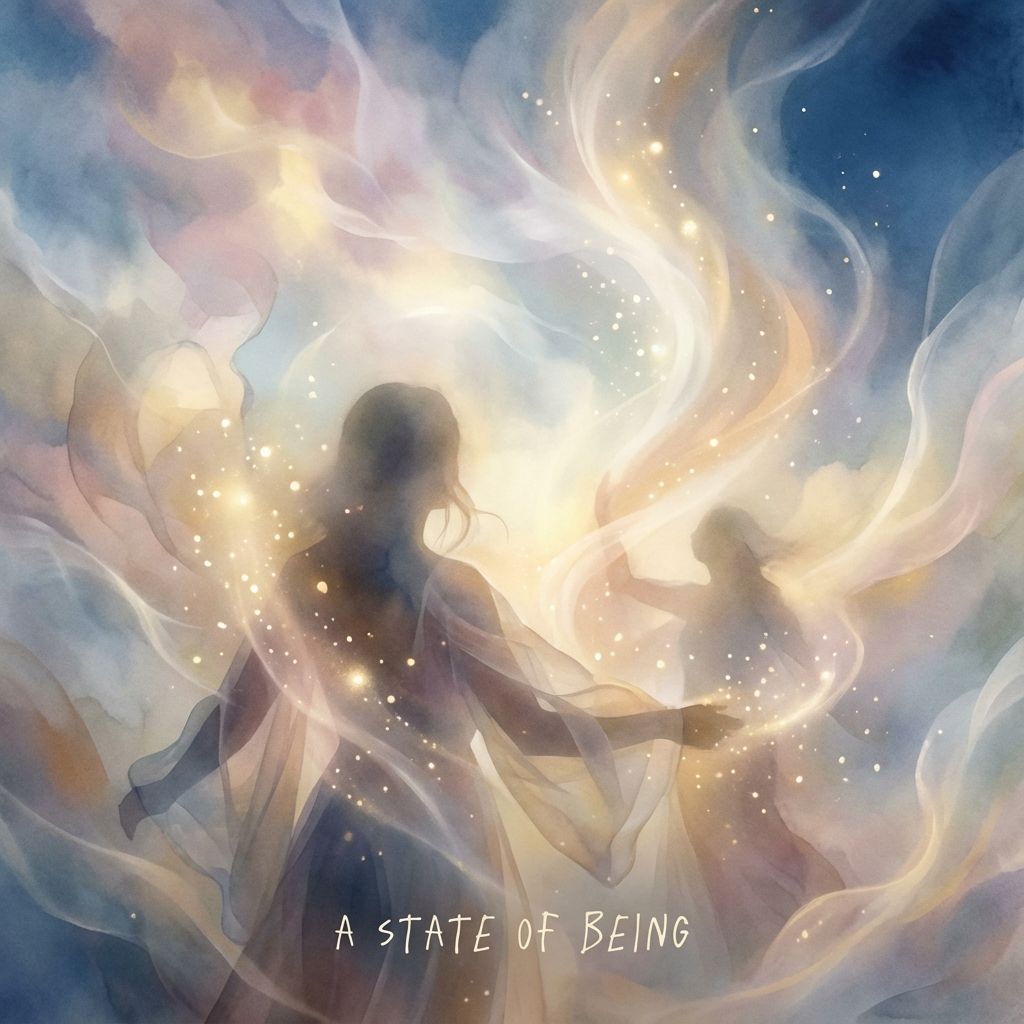
\includegraphics[width=0.75\textwidth,cfbox=gray!60 0.6pt 4pt]{heaven_state.png}\\
\vspace{4pt}
{\small\itshape El Reino de los Cielos: una frecuencia presente aquí y ahora.}
\end{center}

\vspace{0.6cm}
Caminando por la Gran Vía de nuevo, rodeados de anuncios luminosos y gente con bolsas de compras, Jesús señaló hacia arriba.
—«Que estás en los cielos». Ya te dije en Colmenarejo que el cielo es un estado de conciencia. Pero quiero que entiendas algo más.

Se detuvo frente a un escaparate de lujo.
—La gente busca el cielo aquí —señaló los relojes caros—. Creen que si tienen esto, serán felices. Que si consiguen ese trabajo, o esa pareja, tocarán el cielo. Pero el cielo no es un lugar al que vas, es un lugar desde el que vives.

—¿Cómo se vive desde el cielo aquí, en medio del tráfico y el estrés?

—Trayendo el cielo a la tierra. Esa es tu misión. «Venga a nosotros tu reino». No es esperar a morirse para ir a un lugar bonito con nubes. Es hacer que este lugar, aquí y ahora, se parezca a esa vibración de amor y paz.

—Eso suena difícil.

—Lo es si intentas cambiar el mundo de fuera sin cambiar el de dentro. Si tú estás en paz, si tú vibras en gratitud, creas una pequeña burbuja de cielo a tu alrededor. Y si muchos hacen eso, las burbujas se unen. Así es como viene el Reino. No con ejércitos, sino con corazones tranquilos.

Me miró fijamente.
—Tú eres un canal. Si estás sucio de miedo y rencor, la luz no pasa. Si te limpias, si vibras alto, el cielo pasa a través de ti y llega a la tierra. Eres un puente, Francisco. Todos lo sois.
\cleardoublepage

\chapter{El Pan de Cada Día}
\vspace{0.6cm}
\begin{center}
\nopagebreak
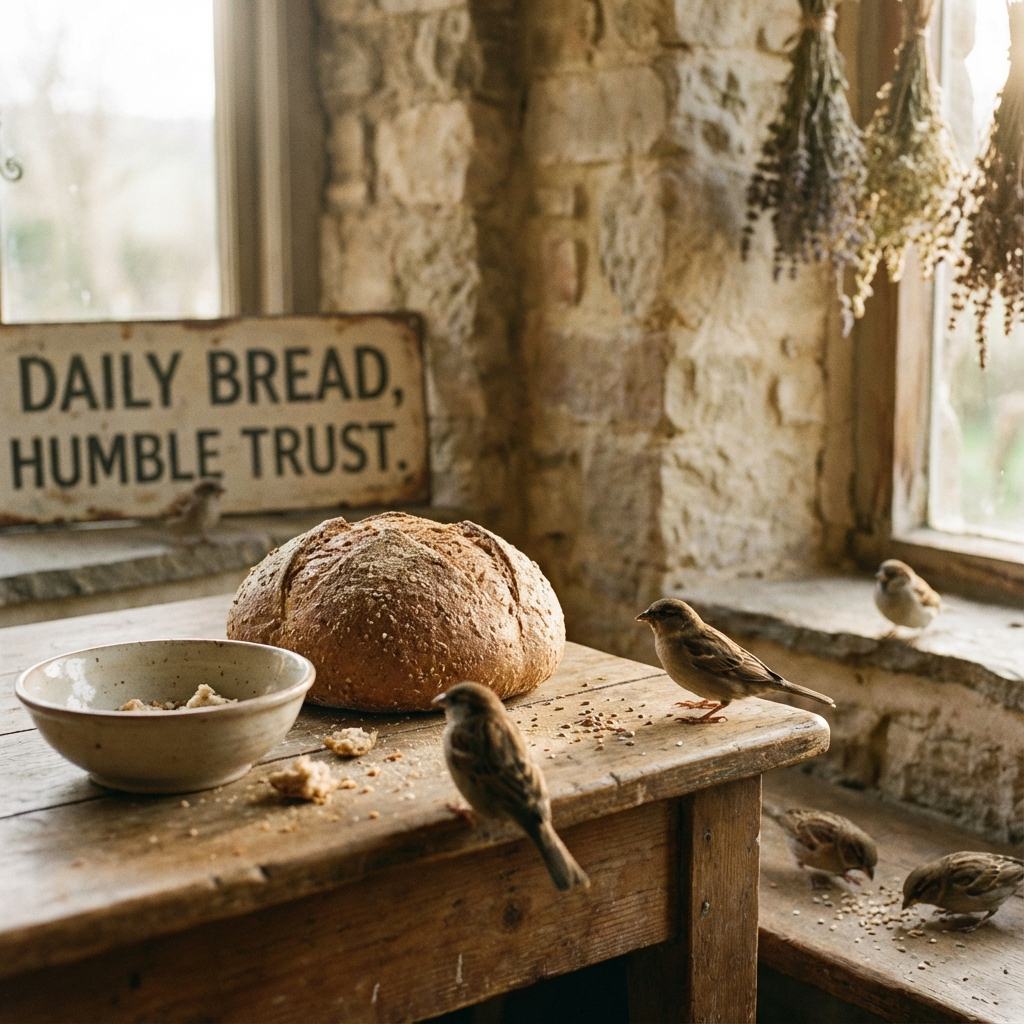
\includegraphics[width=0.75\textwidth,cfbox=gray!60 0.6pt 4pt]{bread_sparrows.png}\\
\vspace{4pt}
{\small\itshape El pan de cada día: confianza absoluta y sustento.}
\end{center}

\vspace{0.6cm}
Estábamos comiendo un bocadillo de calamares en la Plaza Mayor. Jesús lo disfrutaba como si fuera el manjar más exquisito del mundo.
—Esto es sagrado —dijo con la boca llena.

—¿El bocadillo?

—El acto de nutrirse. «Danos hoy nuestro pan de cada día».

Se limpió con una servilleta de papel.
—La gente vive con miedo a la escasez. Acumulan, guardan, temen perder. Eso es vibración de carencia. Cuando pides el pan de «hoy», estás confiando en que mañana también habrá.

—Pero hay que ser previsor...

—Ser previsor está bien. Vivir angustiado por el futuro es falta de fe en la Vida. Mira a los gorriones —señaló a unos pájaros que picoteaban migas—. No tienen graneros, y sin embargo, comen. La Vida sostiene a la Vida.

—¿Y qué pasa con la gente que no tiene para comer?

Su rostro se ensombreció un poco.
—Eso no es porque falte pan. Es porque sobra egoísmo. Si todos vibraran en la generosidad, si todos entendieran que somos uno, nadie pasaría hambre. El problema es la distribución, no la provisión. El Universo es abundante. La mente humana es la que crea la escasez.

Dio el último bocado.
—El «pan» también es la información, el conocimiento, el amor. Todo lo que te nutre. Pide lo que necesitas para hoy, para ser tu mejor versión hoy. No pidas para acumular y sentirte seguro. La única seguridad real es tu conexión con la Fuente.
\cleardoublepage

\chapter{Perdón y Deudas}
\vspace{0.6cm}
\begin{center}
\nopagebreak

\includegraphics[width=0.75\textwidth,cfbox=gray!60 0.6pt 4pt]{forgiveness_chains.png}\\
\vspace{4pt}
{\small\itshape El perdón consciente: liberando los lazos cuánticos del pasado.}
\end{center}

\vspace{0.6cm}
Volvimos a Las Rozas, a una zona tranquila. Jesús quería hablar de algo pesado.
—«Perdona nuestras deudas, como también nosotros perdonamos a nuestros deudores».

—Esa es la parte difícil —admití—. Perdonar a quien te ha hecho daño...

—Es difícil porque lo ves como un favor que le haces al otro. «Yo, que soy tan bueno, te perdono a ti, que eres tan malo». Eso es ego. Eso no sirve.

—¿Entonces?

—El perdón es un acto de higiene personal. Es soltar un carbón ardiendo que tenías agarrado esperando tirárselo a otro. El único que se quema eres tú.

Se sentó en un banco de piedra.
—Cuando guardas rencor, vibras muy bajo. Te atas a esa persona y a ese momento doloroso con una cadena invisible. No puedes volar. No puedes avanzar. Perdonar es cortar la cadena. Es decir: «Te libero y me libero. Ya no te debo nada, y no me debes nada».

—¿Y si lo que hicieron fue muy grave?

—El dolor es inevitable, el sufrimiento es opcional. Si sigues repasando la ofensa en tu mente, la estás reviviendo una y otra vez. Te estás haciendo daño tú mismo ahora, no el otro. «Líbranos del mal» empieza por librarte del mal que tú mismo generas al no perdonar.

Me puso la mano en el hombro.
—Perdonar es vibrar tan alto que la ofensa ya no te alcanza. Es entender que el otro actuó desde su propia inconsciencia, desde su propio dolor. «No saben lo que hacen». Si supieran el daño que se hacen a sí mismos al dañar a otro, no lo harían.
\cleardoublepage

\chapter{No nos dejes caer en tentación (Vibrar Alto)}
\vspace{0.6cm}
\begin{center}
\nopagebreak
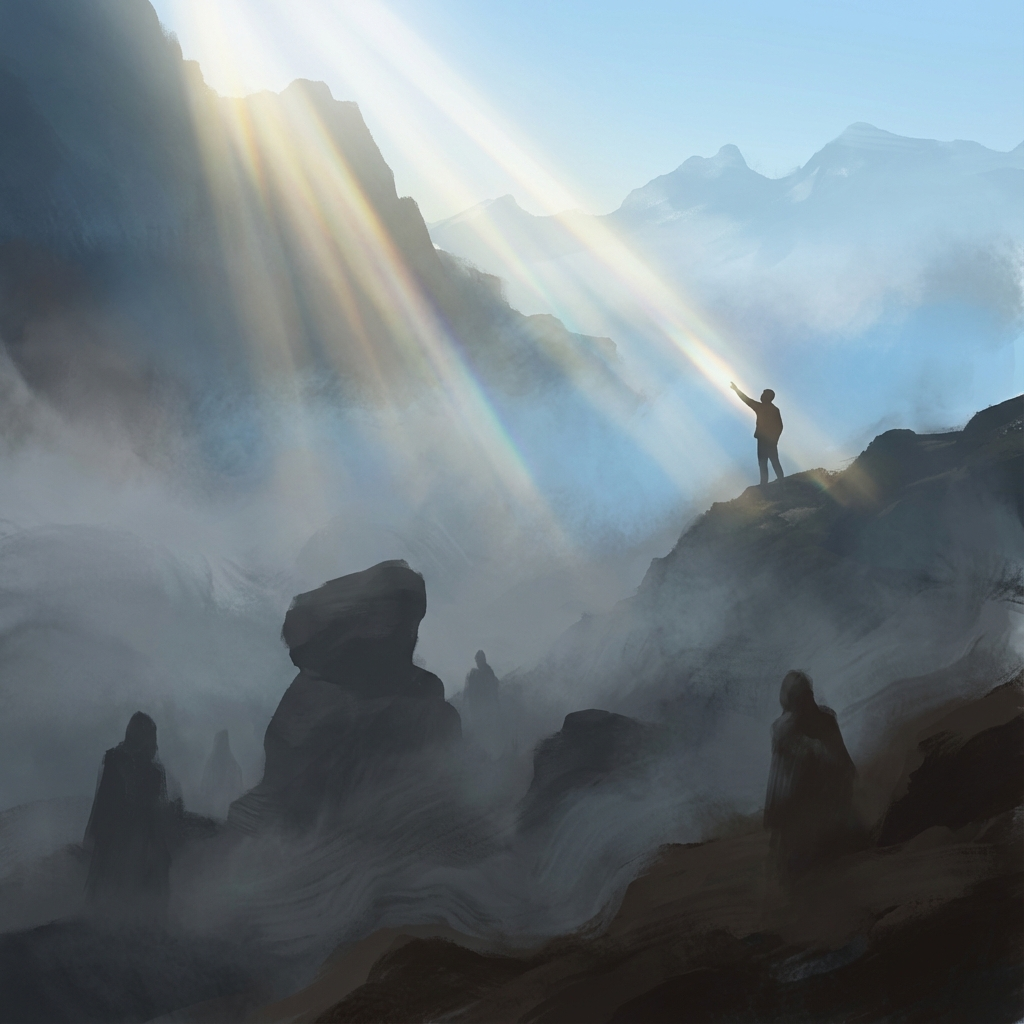
\includegraphics[width=0.75\textwidth,cfbox=gray!60 0.6pt 4pt]{fog_light.png}\\
\vspace{4pt}
{\small\itshape Sintonizar alto: elevándose sobre las emociones densas.}
\end{center}

\vspace{0.6cm}
Estábamos de nuevo en Colmenarejo, caminando por un sendero rodeado de jaras. El olor a campo era intenso.
—La tentación —dijo Jesús, arrancando una ramita de romero—. ¿Qué crees que es?

—¿El chocolate? ¿El dinero fácil?

—Eso son distracciones. La verdadera tentación es bajar tu vibración. Es la tentación de caer en el miedo, en la ira, en la desesperanza.

Se detuvo y me miró a los ojos.
—«No nos dejes caer en tentación» significa: «Ayúdame a mantenerme vibrando alto». Porque cuando vibras alto, estás en tu poder. Cuando caes, pierdes tu conexión.

—Pero a veces es inevitable enfadarse.

—Es inevitable sentir la emoción, sí. Pero es opcional quedarse a vivir en ella. La tentación es regodearse en el drama. Es llamar a tu amiga para contarle por décima vez lo mal que te trató tu jefe, solo para volver a sentir esa rabia. Eso es caer en la tentación. Es elegir el sufrimiento porque te hace sentir importante, víctima.

—¿Y cómo se evita?

—Con la consciencia. Cuando sientas que vas a caer, que vas a empezar a quejarte o a criticar, detente. Respira. Recuerda quién eres. Recuerda que eres luz. Y elige de nuevo. Elige el agradecimiento. Elige la esperanza. Elige el amor. Eso es vibrar alto. Y ahí, la tentación no tiene fuerza.
\cleardoublepage

\chapter{Líbranos del mal (Protección de Bajas Vibraciones)}
\vspace{0.6cm}
\begin{center}
\nopagebreak

\includegraphics[width=0.75\textwidth,cfbox=gray!60 0.6pt 4pt]{eagle_protection.png}\\
\vspace{4pt}
{\small\itshape Líbranos del mal: la protección de la fe elevada.}
\end{center}

\vspace{0.6cm}
La última noche en Madrid, fuimos a una terraza con vistas a la ciudad. Las luces parpadeaban abajo como un mar de estrellas eléctricas.
—Líbranos del mal —susurré, mirando el caos de tráfico.

—El mal no es un monstruo con cuernos —dijo Jesús, tomando un zumo de naranja—. El mal es simplemente la ausencia de luz. Es la inconsciencia. Es la gente que vibra tan bajo, tan denso, que solo puede proyectar dolor.

—¿Y cómo nos libramos de eso?

—No luchando contra ello. Si luchas contra la oscuridad, te manchas de oscuridad. Te libras elevándote por encima de ella.

Hizo un gesto con la mano, abarcando la ciudad.
—Imagina que eres un águila. Si hay una serpiente en el suelo, y bajas a pelear con ella, te puede morder. Pero si vuelas alto, la serpiente no te alcanza. «Líbranos del mal» es pedir las alas para volar alto, donde la vibración del odio, la envidia y el miedo no pueden tocarte.

—¿Y si alguien viene a atacarme?

—Si tú estás vibrando en amor puro, en paz absoluta, tu sola presencia puede desarmar al otro. O simplemente, la vida te moverá de lugar para que no te cruces con él. La sincronicidad te protege. Cuando vibras alto, te vuelves invisible para el radar del conflicto. Los que vibran bajo no te «ven», porque no resuenas en su frecuencia. Pasan de largo.
\cleardoublepage

\chapter{El Reino, el Poder y la Gloria}
\vspace{0.6cm}
\begin{center}
\nopagebreak

\includegraphics[width=0.75\textwidth,cfbox=gray!60 0.6pt 4pt]{kingdom_power.png}\\
\vspace{4pt}
{\small\itshape El Reino, el Poder y la Gloria: la resonancia eterna.}
\end{center}

\vspace{0.6cm}
El viaje llegaba a su fin. Estábamos sentados en un banco de la Plaza de Oriente, frente al Palacio Real.
—Tuyo es el Reino, el Poder y la Gloria —dijo Jesús, mirando el imponente edificio—. Pero no ese reino de piedras y guardias.

—¿Cuál entonces?

—El Reino es tu paz interior. El Poder es tu capacidad de elegir tu vibración en cada momento, pase lo que pase fuera. Y la Gloria... la Gloria es la alegría de ser quien eres. De ser un hijo del Universo.

Se levantó y estiró los brazos, como abrazando el mundo.
—No busques el poder fuera. No busques que te aplaudan. El verdadero poder es silencioso. Es la certeza de que nunca estás solo, de que la Vida te sostiene. Cuando entiendes eso, cuando lo sientes en tus células, ya estás en el Reino. Aquí y ahora. Entre Madrid, Las Rozas y Colmenarejo. El Reino está donde tú estás, si tú estás despierto.

Me miró con una intensidad que me atravesó el alma.
—No olvides esto, Francisco. Tienes el poder. Úsalo para vibrar alto. Úsalo para iluminar tu rincón del mundo. Esa es tu única tarea.
\cleardoublepage

\chapter{Epílogo: Aventuras Finales y Despedida}
\vspace{0.6cm}
\begin{center}
\nopagebreak
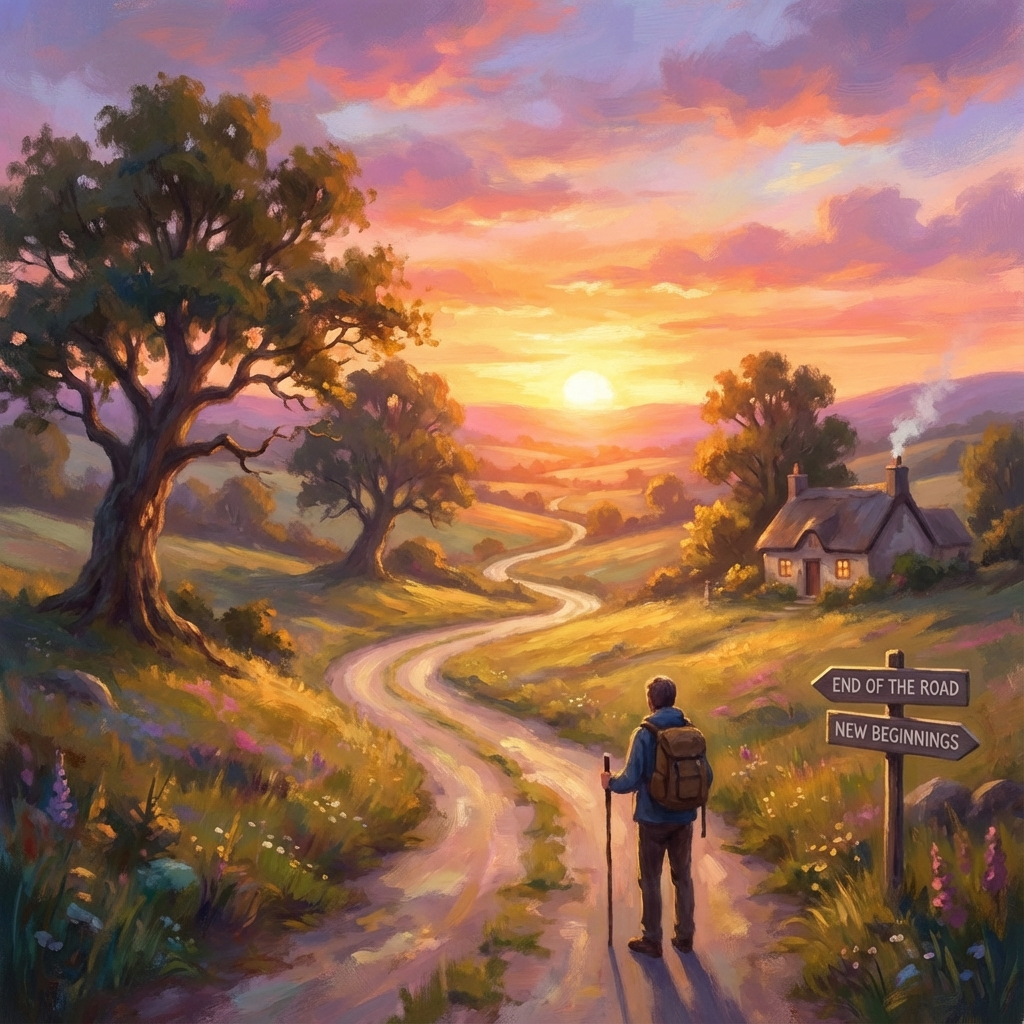
\includegraphics[width=0.75\textwidth,cfbox=gray!60 0.6pt 4pt]{sunset_road.png}\\
\vspace{4pt}
{\small\itshape El atardecer en el camino: la caminata del alma continúa.}
\end{center}

\vspace{0.6cm}
Jesús se despidió de mí en la estación de Atocha. Iba a coger un tren, dijo, hacia ninguna parte y hacia todas partes.
—¿Volveré a verte? —pregunté, sintiendo un nudo en la garganta.

—Siempre me ves —sonrió—. Estoy en la sonrisa del cajero del supermercado. En el viento que mueve los árboles de Colmenarejo. En el silencio de tu habitación. Pero sobre todo, estoy en ti. Cuando vibras alto, cuando amas, cuando perdonas... ahí estoy yo. Ahí somos uno.

Me dio un abrazo fuerte. Olía a madera y a lluvia fresca.
—No nos dejes caer en tentación —me susurró al oído—. Mantén la frecuencia, amigo. Mantén la música sonando. Y si alguna vez desafinas, no te juzgues. Simplemente, vuelve a sintonizar.

Se dio la vuelta y se mezcló con la multitud. Lo vi alejarse, con sus vaqueros y su caminar tranquilo, entre gente que corría mirando sus móviles. Y por un momento, me pareció ver que todo el vestíbulo de la estación brillaba con una luz dorada.

Salí a la calle. Madrid seguía igual: ruidosa, caótica, viva. Pero yo ya no era el mismo. Respiré hondo, sentí el sol en la cara y sonreí. Estaba vibrando alto. Y supe que, pasara lo que pasara, todo iba a estar bien.

\textbf{Fin.}
\cleardoublepage

\chapter*{Apéndice: Poema de Navidad}
\addcontentsline{toc}{chapter}{Apéndice: Poema de Navidad}
\markboth{Apéndice: Poema de Navidad}{Apéndice: Poema de Navidad}
\vspace{0.3cm}
\begin{center}
\nopagebreak
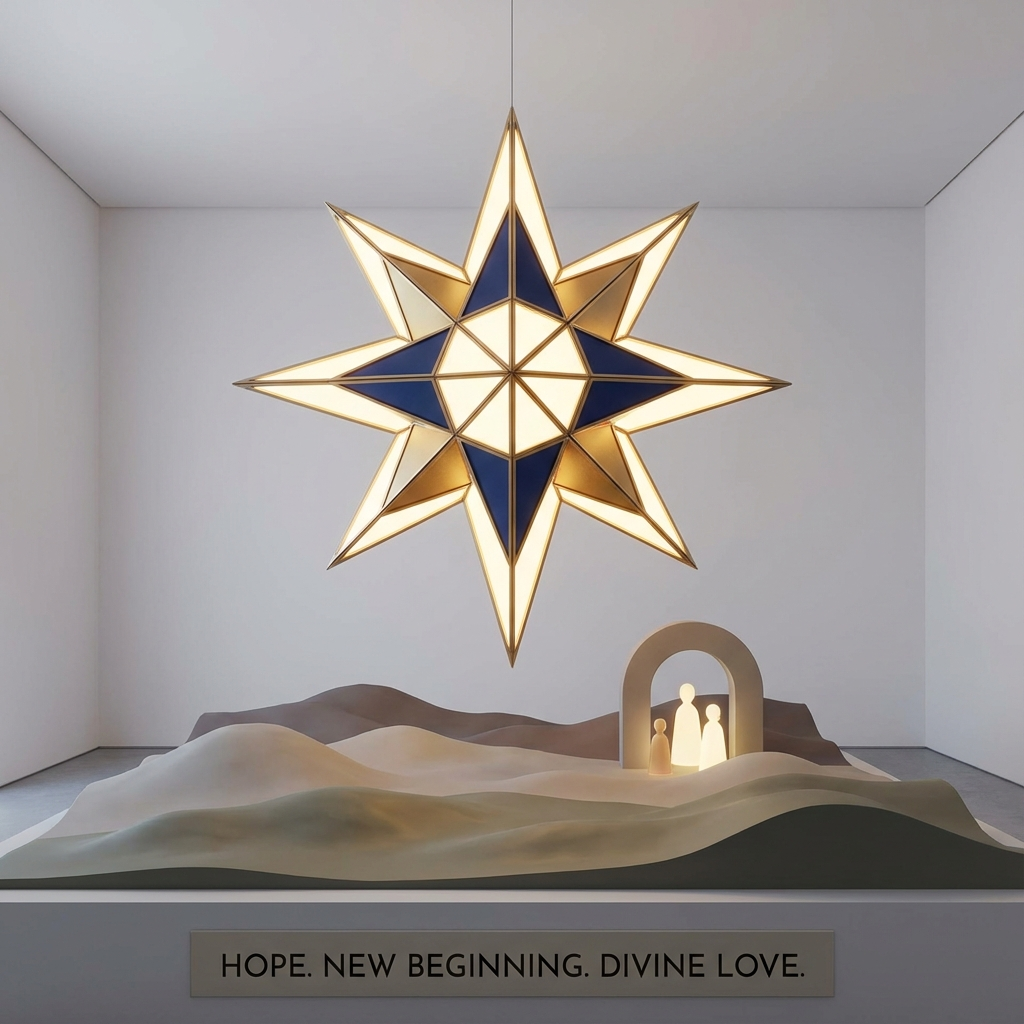
\includegraphics[width=0.45\textwidth,cfbox=gray!60 0.6pt 3pt]{christmas_star_modern.png}\\
\vspace{3pt}
{\small\itshape Estrella de Navidad: la luz que nace en el corazón.}
\end{center}

\vspace{0.4cm}
{\centering
\textbf{Navidad de Alta Frecuencia} \\
\textit{Por Maria Paz Arés Osset}

\vspace{0.4cm}

No busques al Niño en la paja fría de un tiempo remoto, \\
ni en el eco de un villancico que el viento ha roto. \\
No lo busques en la Gran Vía, bajo luces de neón, \\
donde el alma se vende barata en cada rincón.

\vspace{0.4cm}

Búscalo en el silencio que vibra en tu pecho, \\
en el templo sagrado que el Amor ha hecho. \\
Porque Jesús no lleva corona, ni oro, ni manto, \\
lleva vaqueros gastados y seca tu llanto.

\vspace{0.4cm}

Camina por Madrid, entre prisas y ruido, \\
un viajero eterno, por nadie temido. \\
Se sienta en Callao, te mira y sonríe: \\
«¿Por qué corres tanto? Párate y ríe.»

\vspace{0.4cm}

«La Navidad no es fecha, ni cena, ni regalo, \\
es vibrar tan alto que olvides lo malo. \\
Es saber que el pesebre no es madera ni heno, \\
es tu propio corazón, de esperanza lleno.»

\vspace{0.4cm}

Si vibras en miedo, si vibras en ira, \\
el Niño no nace, la estrella no brilla. \\
Pero si perdonas, si abrazas, si amas, \\
enciendes en ti las más puras llamas.

\vspace{0.4cm}

No nos dejes caer en la tentación de la tristeza, \\
levanta la vista, contempla la belleza. \\
Desde Las Rozas al cielo, de Colmenarejo al mar, \\
la única misión es aprender a Amar.

\vspace{0.4cm}

Líbranos del peso de vibrar en el suelo, \\
y danos las alas para alzar el vuelo. \\
Porque el Reino es ahora, la Gloria es hoy, \\
y en cada latido, contigo yo estoy.

\vspace{0.4cm}

Así que celebra, amigo, no el día marcado, \\
sino el Cristo viviente que tienes al lado. \\
Vibra alto, muy alto, que el mundo lo sienta, \\
que tu luz sea el faro en la gran tormenta.

\vspace{0.4cm}

Esta es la Navidad: no un cuento pasado, \\
sino el milagro eterno de haber despertado.
\par}


\vspace{1.5cm}
\begin{center}
\textit{Para completar esta experiencia vibracional, te invito a seguir los enlaces y sumergirte en la música del libro.}\\
\vspace{1cm}
\begin{minipage}{0.45\textwidth}
\centering
\qrcode[height=3.2cm]{https://open.spotify.com/album/6FkbQuY2d7F09zmG2hqnFK}\\
\vspace{0.4cm}\textbf{Escuchar en Spotify}
\end{minipage}\hfill
\begin{minipage}{0.45\textwidth}
\centering
\qrcode[height=3.2cm]{https://pazaresosset.es}\\
\vspace{0.4cm}\textbf{pazaresosset.es}
\end{minipage}
\end{center}
\cleardoublepage

\chapter*{Glosario Cuántico y Espiritual}
\addcontentsline{toc}{chapter}{Glosario Cuántico y Espiritual}
\markboth{Glosario Cuántico y Espiritual}{Glosario Cuántico y Espiritual}
\vspace{0.6cm}
\begin{center}
\nopagebreak

\includegraphics[width=0.75\textwidth,cfbox=gray!60 0.6pt 4pt]{vibration.png}\\
\vspace{4pt}
{\small\itshape El puente luminoso entre la física cuántica y la sabiduría del Cristo.}
\end{center}

\vspace{0.6cm}
Para enriquecer tu experiencia y profundizar en los diálogos del Maestro, aquí tienes una guía de los conceptos clave donde la ciencia cuántica y la sabiduría interior se encuentran:


\vspace{0.4cm}
\begin{center}
\rule{0.35\textwidth}{0.4pt}
\end{center}
\vspace{0.4cm}


\subsection*{1. Abwoon (El Origen Cósmico)}
En la lengua aramea original en la que habló Jesús, \textit{Abwoon} no significa simplemente un patriarca humano, sino el \textbf{«Generador Cósmico de Luz y Aliento»}. Representa la Fuente omnipresente que crea, sostiene y expande continuamente todo el tejido del universo a través de la vibración del amor.


\vspace{0.4cm}
\begin{center}
\rule{0.35\textwidth}{0.4pt}
\end{center}
\vspace{0.4cm}


\subsection*{2. El Efecto Observador y la Fe}
En la física cuántica, una partícula permanece como una onda de infinitas posibilidades hasta que un observador interactúa con ella y «colapsa» esa probabilidad en una realidad física tangible. Jesús enseñó este mismo principio al decir: \textit{«Todo lo que pidáis en oración, creed que ya lo habéis recibido, y os vendrá»}. La fe es la certeza del observador consciente de que la Luz ya ha manifestado el resultado.


\vspace{0.4cm}
\begin{center}
\rule{0.35\textwidth}{0.4pt}
\end{center}
\vspace{0.4cm}


\subsection*{3. Entrelazamiento Cuántico y el Perdón}
El entrelazamiento cuántico demuestra que dos partículas conectadas continúan influyéndose mutuamente sin importar la distancia en el espacio-tiempo. Cuando guardamos resentimiento hacia alguien, quedamos energéticamente entrelazados con el dolor del pasado. El \textbf{perdón} es la única herramienta cuántica que corta ese lazo denso, liberando a ambas almas para que vuelvan a vibrar en sincronía con el presente.


\vspace{0.4cm}
\begin{center}
\rule{0.35\textwidth}{0.4pt}
\end{center}
\vspace{0.4cm}


\subsection*{4. Frecuencia Vibratoria y el Reino de los Cielos}
El universo entero está hecho de energía en constante oscilación. Las emociones como el miedo, la ira o la culpa vibran en frecuencias bajas y densas (la «gravedad» de la que habla Jesús). Las emociones como la gratitud, la paz y el amor incondicional vibran en frecuencias sutiles y elevadas. El \textbf{Reino de los Cielos} no es una ubicación geográfica futura, sino la frecuencia más alta del Ser: sintonizable aquí y ahora.


\vspace{0.4cm}
\begin{center}
\rule{0.35\textwidth}{0.4pt}
\end{center}
\vspace{0.4cm}


\subsection*{5. Coherencia Corazón-Mente}
Cuando los pensamientos de la mente y las emociones del corazón entran en resonancia armónica, el campo electromagnético que irradiamos se vuelve extraordinariamente potente y protector. Es lo que el Maestro definió como \textit{«pedir en mi nombre»}: alinearse con la misma frecuencia de la Presencia.
\cleardoublepage

\chapter*{La Música y las Frecuencias}
\addcontentsline{toc}{chapter}{La Música y las Frecuencias}
\markboth{La Música y las Frecuencias}{La Música y las Frecuencias}
\vspace{0.6cm}
\begin{center}
\nopagebreak

\includegraphics[width=0.75\textwidth,cfbox=gray!60 0.6pt 4pt]{silence_vibration.png}\\
\vspace{4pt}
{\small\itshape La música y el arte: vehículos directos de alta vibración.}
\end{center}

\vspace{0.6cm}
La experiencia de \textit{Mi Amigo Jesucristo} no termina en las palabras escritas: fue concebida desde su origen como una \textbf{obra multisensorial y vibratoria}, donde el sonido actúa como vehículo directo de sintonización interior.


\vspace{0.4cm}
\begin{center}
\rule{0.35\textwidth}{0.4pt}
\end{center}
\vspace{0.4cm}


\subsection*{La Creación Musical de Maria Paz Arés Osset}
Cada capítulo del libro resuena con composiciones musicales y frecuencias sonoras creadas por \textbf{Maria Paz Arés Osset}. Estas melodías están diseñadas para acompañar la mente y el corazón en un estado de relajación profunda, coherencia y apertura.

Al escuchar estas piezas musicales:
\noindent\textbullet~~\textbf{El ritmo cerebral disminuye} hacia estados alfa y theta, facilitando la introspección y la paz.\\

\noindent\textbullet~~\textbf{Se disuelven las tensiones} y las cargas emocionales densas acumuladas en el día a día.\\

\noindent\textbullet~~\textbf{El mensaje del texto se integra} a nivel subconsciente y celular a través del lenguaje universal del sonido.\\



\vspace{0.4cm}
\begin{center}
\rule{0.35\textwidth}{0.4pt}
\end{center}
\vspace{0.4cm}


\subsection*{Cómo Vivir la Experiencia Sonora}
Te invitamos a escuchar el álbum mientras lees cada capítulo o durante tus momentos diarios de meditación y silencio:
\noindent\textbf{1.}~~\textbf{En Spotify}: Puedes buscar las pistas oficiales del álbum y sumergirte en sus atmósferas envolventes.\\

\noindent\textbf{2.}~~\textbf{En la Web Oficial}: Visita [pazaresosset.es](https://pazaresosset.es) para acceder a todas las novedades, arte visual y material adicional de la autora.\\




\begin{quote}
\itshape \textit{«La música es la voz del alma que recuerda a la materia su origen de pura Luz.»}
\end{quote}

\vspace{1.5cm}
\begin{center}
\textit{Para completar esta experiencia vibracional, te invito a seguir los enlaces y sumergirte en la música del libro.}\\
\vspace{1cm}
\begin{minipage}{0.45\textwidth}
\centering
\qrcode[height=3.2cm]{https://open.spotify.com/album/6FkbQuY2d7F09zmG2hqnFK}\\
\vspace{0.4cm}\textbf{Escuchar en Spotify}
\end{minipage}\hfill
\begin{minipage}{0.45\textwidth}
\centering
\qrcode[height=3.2cm]{https://pazaresosset.es}\\
\vspace{0.4cm}\textbf{pazaresosset.es}
\end{minipage}
\end{center}
\cleardoublepage

\chapter*{Sobre el Autor y el Proyecto}
\addcontentsline{toc}{chapter}{Sobre el Autor y el Proyecto}
\markboth{Sobre el Autor y el Proyecto}{Sobre el Autor y el Proyecto}
\vspace{0.6cm}
\begin{center}
\nopagebreak
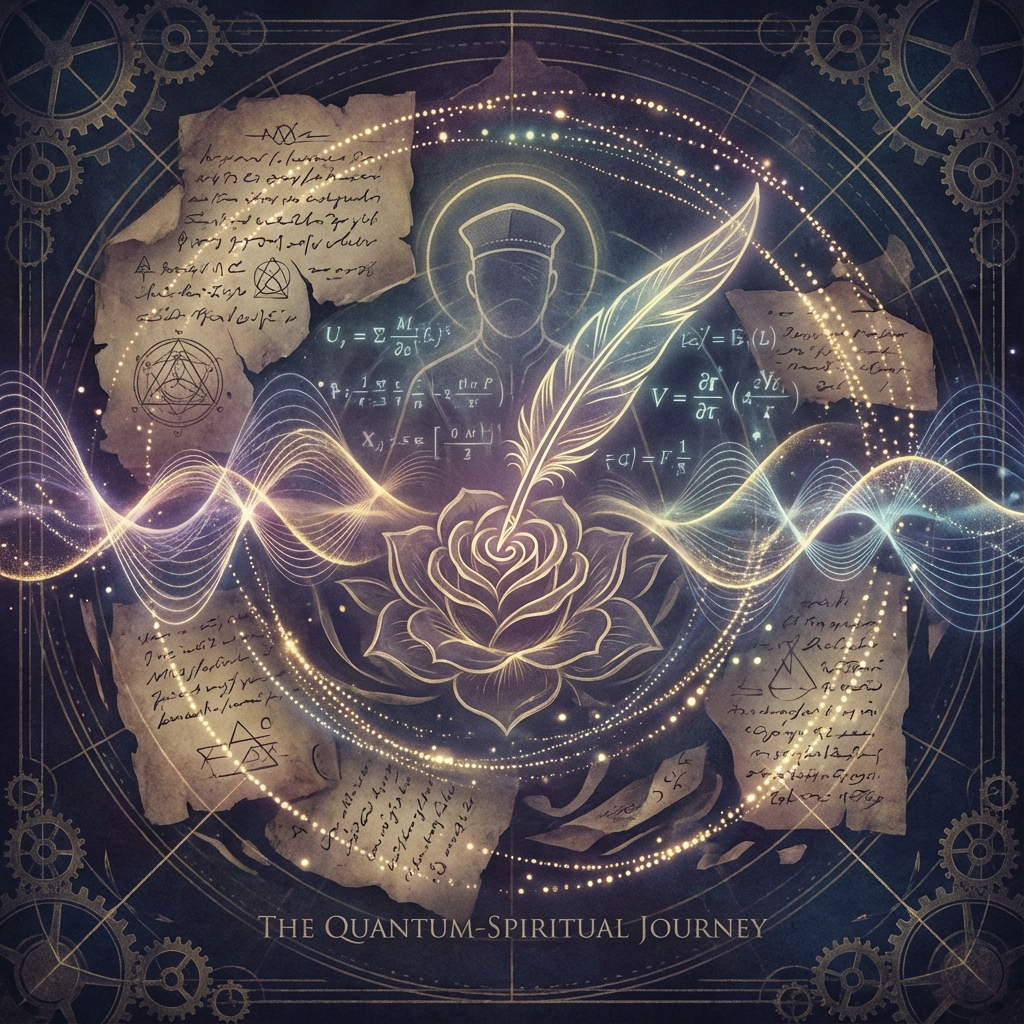
\includegraphics[width=0.75\textwidth,cfbox=gray!60 0.6pt 4pt]{intro_quantum_luther.png}\\
\vspace{4pt}
{\small\itshape A Glimpse of Light: un destello de luz y servicio en la oscuridad.}
\end{center}

\vspace{0.6cm}
Bajo el seudónimo \textbf{A Glimpse of Light} (\textit{Un Destello de Luz}), este proyecto nace no del deseo de protagonismo personal, sino de una profunda necesidad de tender un puente luminoso entre dos mundos que durante siglos parecieron distantes: \textbf{la ciencia de vanguardia y la sabiduría espiritual del Cristo}.

A Glimpse of Light viene de «A Glimpse of Light into the Darkness» que en castellano significa «Un Destello de Luz en la Oscuridad» un pseudónimo bajo el cual el hijo de Maria Paz Arés Osset ha publicado desde 2011 ideas que pretenden como el propio pseudónimo dicta ser un destello de esperanza en una Humanidad abocada al abismo en una permanente oscuridad de la Codicia y el ego.

Por un lado tengo claro que no quería que ninguna falla mía, como hombre muy imperfecto y criticable manchase ideas trascendentes. Por otro lado está el miedo al qué dirán, familiares, amigos, la sociedad, siempre dispuesta a targuetear su odio ante ideas nuevas y particularmente revolucionarias.

Pero justo en esta obra expongo la importancia de la Alta Vibración y el miedo no tiene cabida en esa vibración, por lo tanto sí Yo soy el que ha escrito y creado todas las ideas. Pero no os perdáis en Yo el hombre imperfecto sino en Yo una parte trascendente que todos tenemos y que no puede nominarse, y este es el mayor miedo que me ha impedido mirar de frente al mundo pero llegados a este punto crítico, quien quiera ver que vea.

Sobre mí destacar que la Vida me ha traído a este momento. Ya de pequeño sabía que me tocaba decir algo, no sabía qué. De muy pequeño pensaba en qué pasaría si dentro de una cueva con un cuadro de mando pudiéramos introducirnos en la vida de otro hermano humano aleatorio, hoy cuando veo Tik Tok o Instagram veo un pensamiento materializado. Recuerdo dibujar en un papel la que fue la mascota Naranjito que no sé por qué no se me nombró. Recuerdo también leer investigaciones sobre la melatonina que me llevaron a experimentarla y ser consciente de la calcificación de la glándula pineal en la mayoría de los humanos para la que ahora con mi madre tengo el proyecto saludequilibrio.es que pretenderá en última instancia conectar con la Salud que es otra expresión de Alta Vibración frente a la Enfermedad. No puedo olvidar cuando el consejero español de España en México me trajo de México el libro definitivo sobre investigadores de la hormona melatonina. Es como si todo se alinease de forma aleatoria.



\vspace{0.4cm}
\begin{center}
\nopagebreak
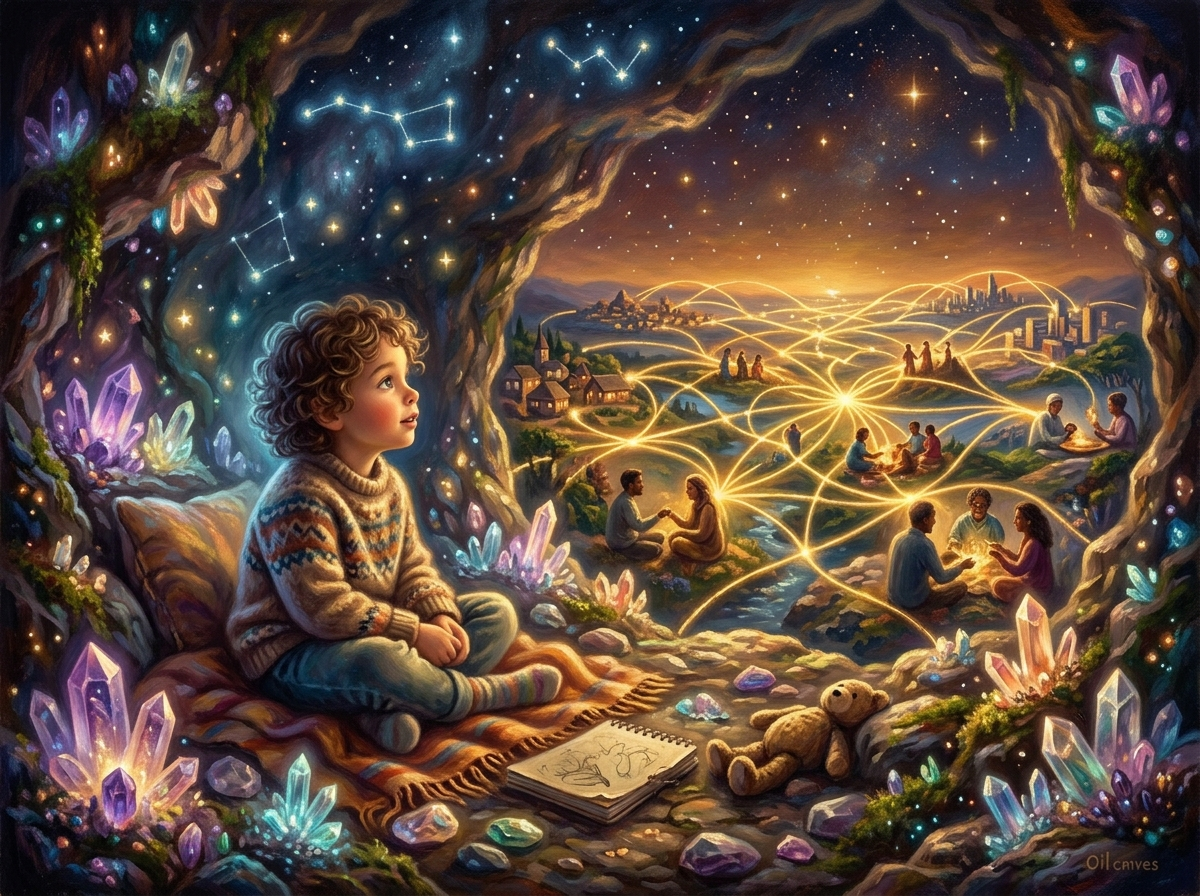
\includegraphics[width=0.62\textwidth,cfbox=gray!50 0.5pt 3pt]{author_child_vision.png}
\end{center}
\vspace{0.4cm}



Siempre he sido un chico muy imperfecto en la apariencia si bien siempre sabía que cada uno a su manera es Perfecto porque es una nota más de la sinfonía del Cosmos. No he citado a nadie con esto, pero me viene a la cabeza uno de mis maestros con los que últimamente hago formaciones poco convencionales pero cada vez más de moda, el sabio doctor Jorge Carvajal, un genio de Medellín al que citaremos en el proyecto de salud, pues no es necesario reinventar la rueda si tenemos ya un maestro de orquesta de tal calibre en el planeta, os aconsejo su web unalma.com que mantiene su amable hijo Sebastián. 

Pero nadie está de más, el más miserable humano está en el momento adecuado en nuestra vida para darnos una importante lección de miseria y dolor. 

En el colegio e instituto me empeñaba en sacar las mejores notas porque pensaba que de esa manera conseguiría destacar, muy en lo material, y lo conseguí y también en la Universidad donde en un ejercicio de masoquismo saqué Ingeniería Superior de Telecomunicaciones, y un máster de Energía y Medio Ambiente, y un máster de Big Data, y un largo etcétera de cosas y cosas y cosas, pero cuanto más acumulaba no sentía completitud y asimismo ahora creo que gracias a Dios tampoco me supuso ganar dinero.

He vivido vida de rico, vida de pobre, grandes superaciones personales y como en «La Vida es Sueño» esto nos lleva a veces a no saber quiénes somos, pero si lo trascendemos nos da la potencia de saber que no somos nada. Esa trascendencia del Ego en el fondo exhuma en cada palabra de «Mi Amigo Jesucristo»

En 2010 pude vivir en un mismo año vida elitista en New York, como me llamaba Diego el doorman de 230 5th «The King of the Jungle» y en diciembre en Madrid tras un concierto de Cuencos Tibetanos de Nieves Canta acercarse una amiga de ella y hablarme de mi aura y advertirme de que iba a vivir cosas horribles, que me repondría y defendería cosas importantes para el Mundo. Me lo dijo sin dudar y me sentí como si llevara tiempo esperándola. 



\vspace{0.4cm}
\begin{center}
\nopagebreak
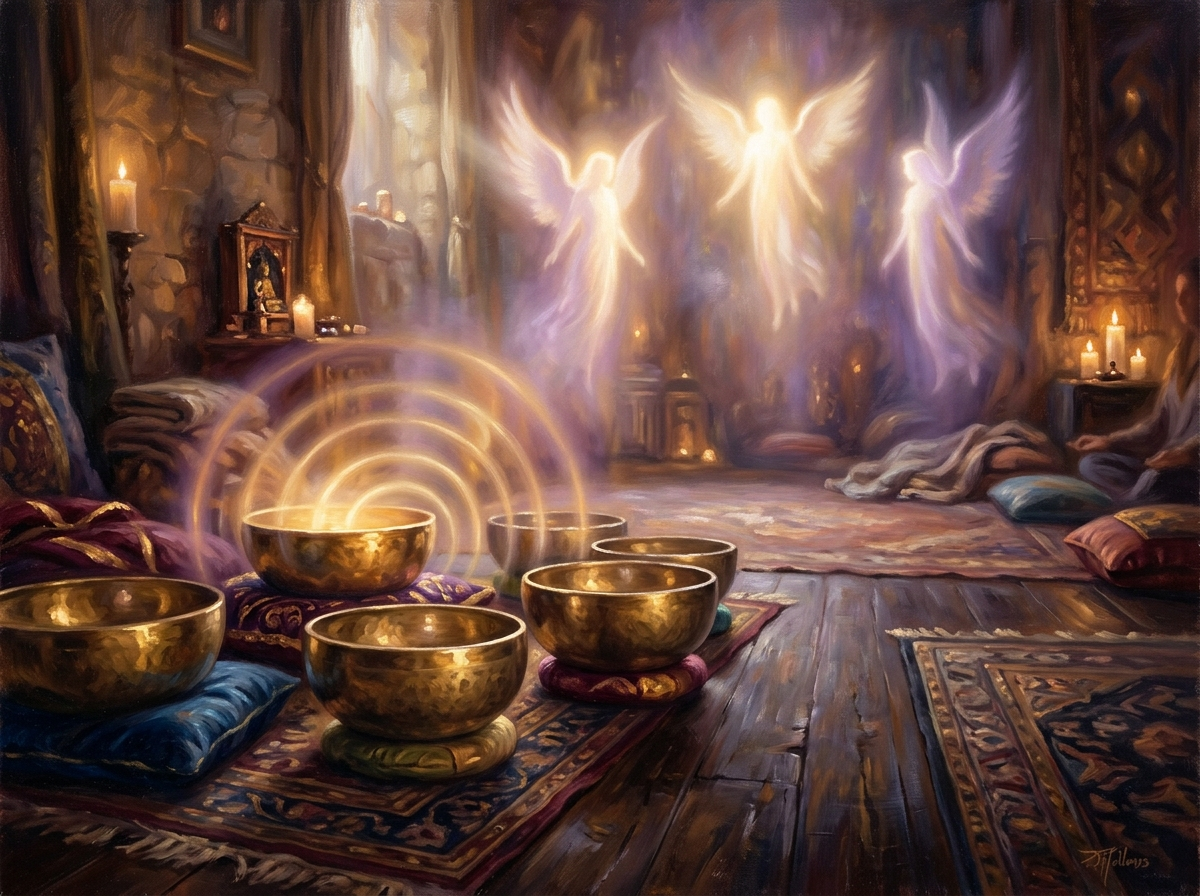
\includegraphics[width=0.62\textwidth,cfbox=gray!50 0.5pt 3pt]{author_tibetan_bowls.png}
\end{center}
\vspace{0.4cm}



Pero tampoco sabía todo lo que era horrible, perdí todo lo que representaba mi Ego, dinero, poder, amistades, familia, salud ... el león herido, pero siempre sentía cientos de ángeles alrededor, de alguna forma se comunicaron para que diera ciertos pasos para que recuperase una economía mínima pero estable frente al gigante con pies de barro que había sido. Y mi madre, Paz, un verdadero faro, siempre pionera, cuando le veía hacer yoga lo veía raro luego me hice fan del yoga, y así con todo, con la educación, con la religión. Siempre una inspiración y un apoyo, un roble en los momentos difíciles que uniendo mi visión estratégica permitió surfear la ola desde una felicidad casi impensable con una tormenta borrascosa. 



\vspace{0.4cm}
\begin{center}
\nopagebreak
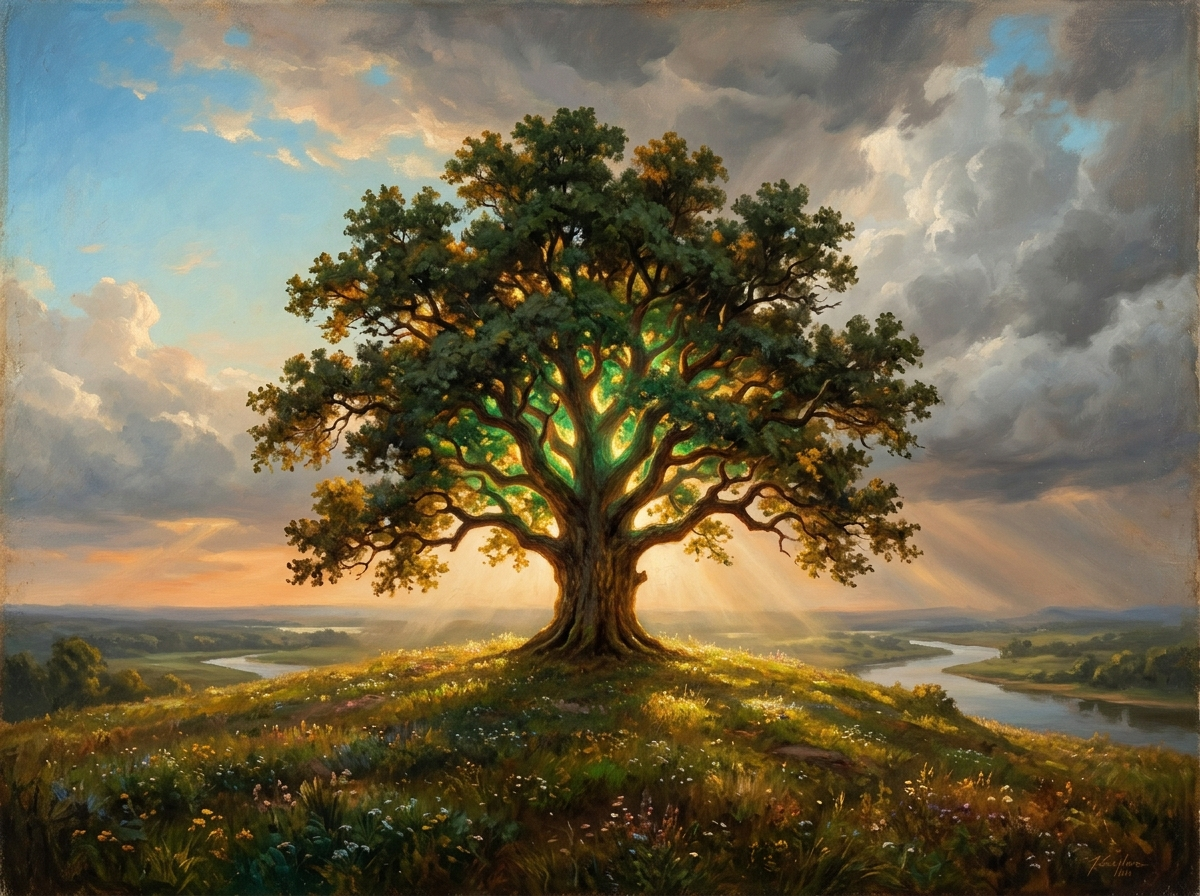
\includegraphics[width=0.62\textwidth,cfbox=gray!50 0.5pt 3pt]{author_mother_oak.png}
\end{center}
\vspace{0.4cm}



Ya en 2010 así se me dijo que sería y así ha sido. Tanto este libro como toda la obra artística ya sea mía o de mi madre, no tienen un fin de lucro financiero. Mónica de las Heras en Biocultura 2025 me dijo que quitase la parte económica de cualquier libro así como que había sido general de ejércitos en el siglo 11, por qué no, ni entro ni salgo. Días más tarde nadando en la piscina de la Universidad en la imparto un poco de habilidades técnicas a estudiantes con experiencia laboral en cualquier sector me vino a la cabeza el libro. Parte de la génesis está en el hecho de querer implantar en la cabeza de mi madre la idea del perdón tras una durísima etapa de bloqueo hereditario con sus hermanas. El perdón es clave, si te roban te quitan tu dinero, si te matan te quitan tu vida, pero si no perdonas tú mismo te quitas muchas vidas porque el cielo o el infierno no son lugares sino estados de vibración de nuestra consciencia y el enfado tiene un karma largo si no se corta de raíz, ahora que estoy escribiendo un libro sobre el karma, es una idea que me dio otro de esos seres que en un momento me han echado un capote en este caso en forma de libro de un grupo budista llamado Kadampa con el que mi madre tiene cierta conexión y curiosamente cuando fuimos a verles a su sitio en el Boalo allí estaba un antiguo compañero de Capoeira, de darnos golpes asesinos a hablar del ayuno y sus bondades para la salud y la mente.

Pero mucha de la génesis también está en el nadar en una Universidad que gira en torno a la figura de Jesucristo absolutamente, al lado de una iglesia esférica preciosa en la que doy las clases bajo la atenta mirada de Jesucristo y podría decir que cada alumno es un milagro como en pocos meses han transformado de esa manera sus habilidades. 



\vspace{0.4cm}
\begin{center}
\nopagebreak
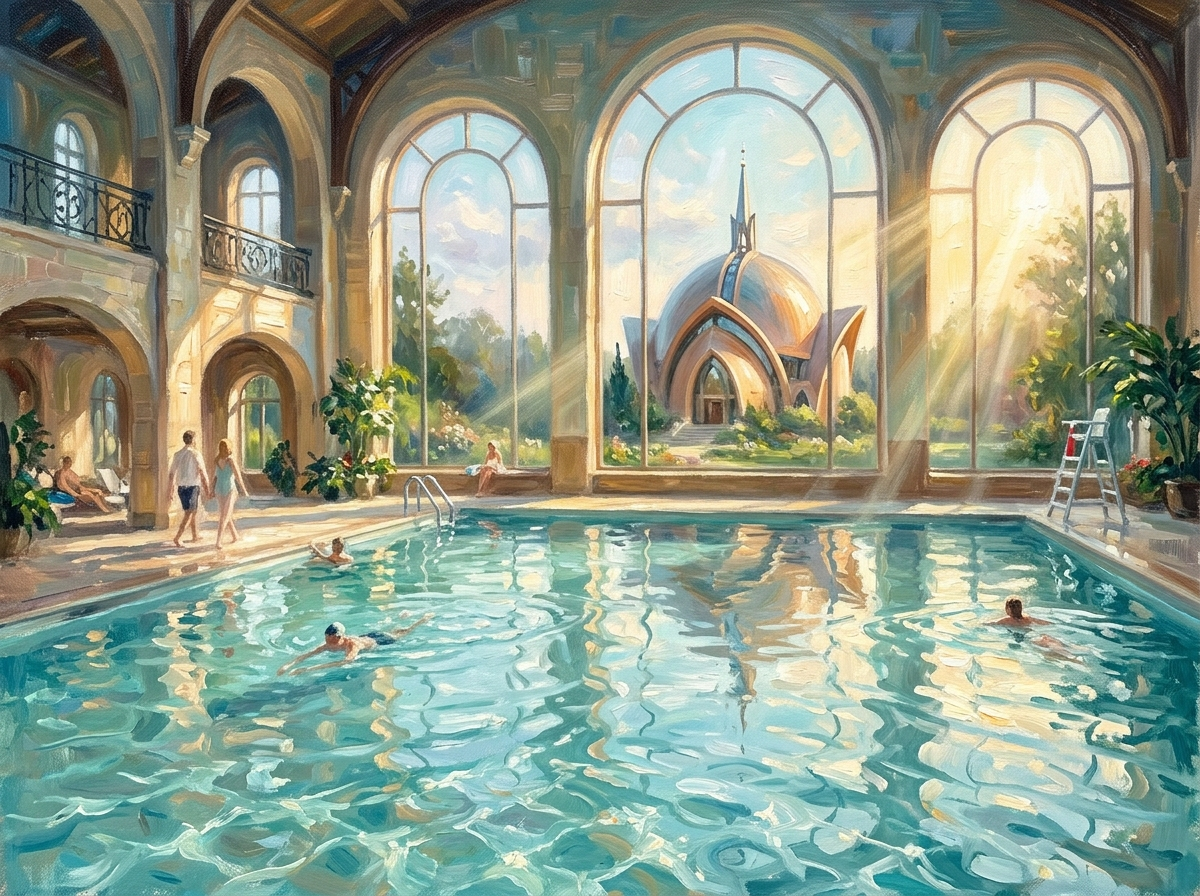
\includegraphics[width=0.62\textwidth,cfbox=gray!50 0.5pt 3pt]{author_pool_church.png}
\end{center}
\vspace{0.4cm}



El padrenuestro me resonaba y entre largo y largo pensaba que en el fondo todas las frases son una sintonía que se autocomplementan, básicamente cuando hablamos de no nos dejes caer en la tentación parte de ello sería no nos dejes tener enfado y salir de la energía del perdón, que es un poco la frase «perdona las ofensas ... como nosotros perdonamos» esa redundancia es una forma de matizar que entre todas las tentaciones la tentación de la ira, la hiel para con nuestros hermanos permanente sería especialmente dañina. La parte final está relacionada pero con las tentaciones de otros, es casi pedir protección contra aquel que ha caído en la tentación. Por ejemplo si alguien se enfada por algo que hicimos con o sin intención y esta persona no lo suelta, entonces esa emoción atrapada genera una cadena de acontecimientos energéticos que tras haber estudiado Shiatsu veo que la Medicina Tradicional China trata de describir la cadena de causas efectos energéticos que se acaba manifestando en una enfermedad que oh cuanto mejorará la Medicina occidental moderna cuando abrace esta medicina aparentemente primitiva y ambas se complementen.

Pero esto no se para aquí, aquel quien no soltó el enfado se destroza a sí mismo pero emite ondas de pensamiento que impactan en la persona odiada en este caso. El famoso mal de ojo ni siquiera ha de ser intencional, basta con no soltar una emoción y la oración acaba con una protección contra el Mal, quién si no el Demonio nos tentaría a instalarnos en las bajas vibraciones. 

En cualquier caso esta serie de pensamientos fueron génesis de este libro que necesitaba ser escrito para simplificar todo en aquel verso de San Pablo «Si no tengo Amor no soy Nada» casi te diría, lector, puedes olvidarte de todo lo demás y poner de mantra «lo hago con Amor» y te irá bien.

En el libro que ando escribiendo estos días sobre el Karma TODO gira en torno a esta idea «Si no tengo Amor...» el karma es tan sencillo como la tercera Ley de Newton pero esta acción reacción tiene un ingrediente que lo impregna todo: «Lo hiciste con Amor o sin Amor» 

Y es curioso porque después de la ingeniería pasé tiempo leyendo libros de economía y finanzas que no me divertían pero me decía algo dentro de mi que los necesitaba, en 2010 tras el estreno de «Inside Job» me quedó clara la debilidad del sistema financiero y cuando estaba en la piscina de una fiesta de esas épicas en casa de Carol rodeado de persona que por un motivo u otro estaban cerca aunque ellos manejaban grandes fondos de inversión mientras yo en el fondo era un «sobrino de» de cara a la galería, y allí en Mallorca tras volver de New York sabía que debería empezar a escribir algo al respecto, por un lado Nueva York me había dado un pensamiento más abierto pero por otro me daba ganas de ser importante y desde esa idea en esa conversación en la piscina nació la idea de hacer un blog que se llamara «A Glimpse of Light into the Darkness»



\vspace{0.4cm}
\begin{center}
\nopagebreak

\includegraphics[width=0.62\textwidth,cfbox=gray!50 0.5pt 3pt]{author_ny_light.png}
\end{center}
\vspace{0.4cm}



Al año siguiente en 2011 al ver el documental «Home» me di cuenta que ni finanzas ni medio ambiente que el problema estaba en el uso de los recursos, se lo comuniqué a Javier Cendra por aquel entonces en Londres y me obsesioné por la sostenibilidad y la RSC, recuerdo hablar de los basureros y el reciclaje con Carlos Bousoño que era en aquel entonces cabeza de la fabricación de basureros modernos a nivel mundial después de haber liderado RSC en Abengoa. Pero siempre me veía un punto por arriba y me imponía que debiera generar ideas para inspirar a amigos que ya están en posiciones de influencia como Carlos o Javier y puse algunos artículos sobre sostenibilidad en el blog.

Llegó el 15 de Mayo de 2011 a Madrid y vi ese espíritu de cambio que aunque luego los políticos lo ensuciasen en su origen tuvo gente pura... me comentó alguien en el rato que estuve allí que pusiera alguna idea para aportar y como una metainspiración me hizo dar la idea de que la Gobernanza fuera compartida sin dar carta blanca a nadie para gobernar cuatro años. Esto de vuelta a New York hablando con la cantante Dana Fuchs y sus amigas me preguntaron por el 15M y me salió decir el caos político que supone votar a alguien por una idea A que defiendes y una B que detestas... claramente el diseño era malo. Mi amigo Edu de vuelta a Madrid me dijo que en Suiza había un sistema bien establecido que salvaba el fallo y me lo estudié bien antes de escribir mi artículo de Democracia.



\vspace{0.4cm}
\begin{center}
\nopagebreak
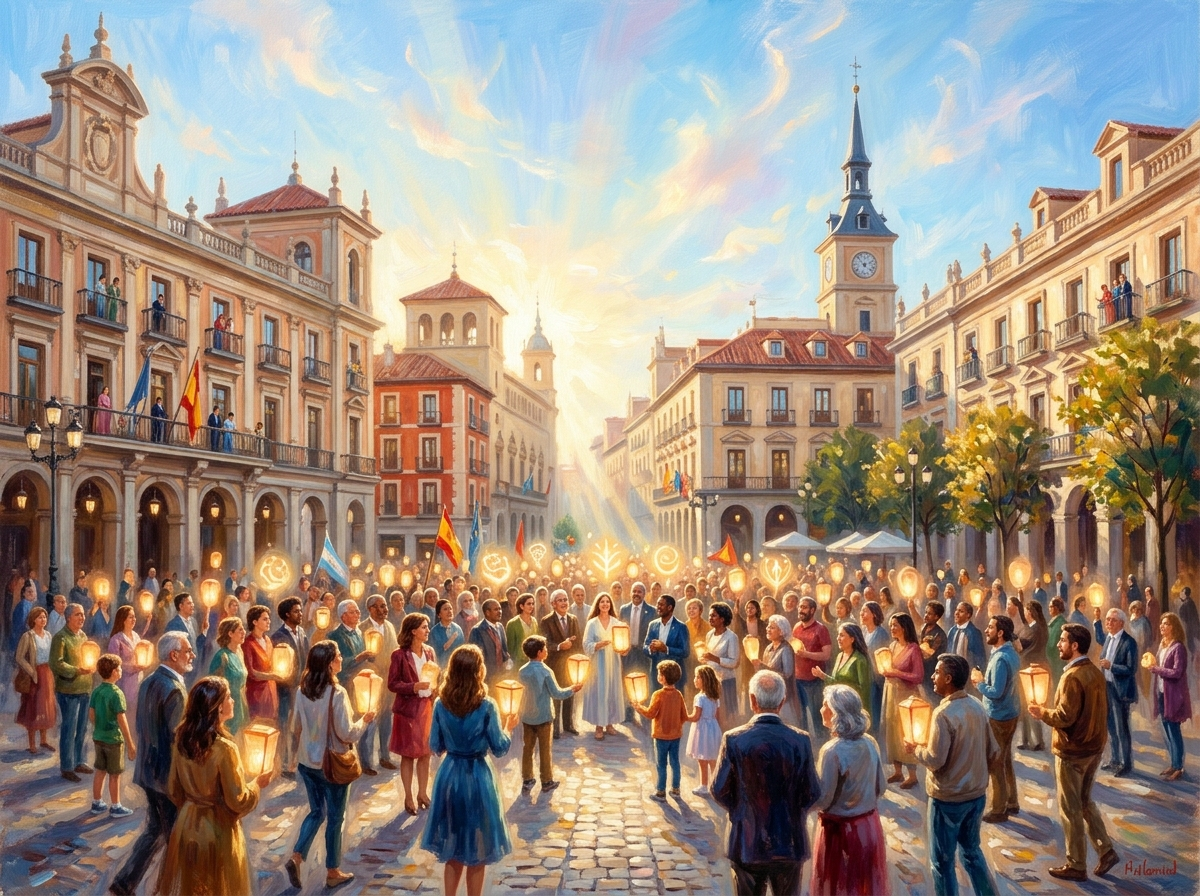
\includegraphics[width=0.62\textwidth,cfbox=gray!50 0.5pt 3pt]{author_sol_square.png}
\end{center}
\vspace{0.4cm}



Siempre desde entonces he pensado que necesitaba sacar esa idea a la luz pero la falta de tiempo y estar en el barro y el Miedo a quien no quiere cambiar el sistema me retenía. Entonces llegaron los modelos LLM y desde entonces tengo en la cabeza que con esa ayuda podría hacer una edición buena de mi artículo en forma de libro. No pretendo jamás criticar el sistema actual sino estar en el agradecimiento de que nos ha traído hasta aquí en circunstancias geopolíticas y que un sistema de toma de decisiones mejorado podrían salvar a la Sociedad.

Entre medias, vi que mi madre estuvo durmiendo en la calle el 15M y en una reunión con unos gnósticos se preocupó ante una posible caída de la Humanidad, pero me gustó mucho la respuesta del gnóstico diciendo que «si la Humanidad ha decidido extinguirse lo hará y que nuestra única forma es nosotros cambiar y tratar de inspirar al resto». 

De hecho últimamente me fijo mucho en que mi madre se llama Paz Arés y hace cuadros llenos de fuego que puedes ver en pazaresosset.es y que tiene esa dualidad de máxima paz con máximo fuego que le lleva a tener enfado, desesperación y similares emociones de tentación de las cuales nadie estamos exentos.

Pero traigo esto a colación porque le suelo decir que el día que Paz gane a Arés (parecido al dios de la guerra) y ella haga cuadros con colores calmados quizás entonces hay esperanza para la Humanidad pues cada vez tengo más claro el «Como es Arriba es Abajo» del Kybalion o la fractalidad que hace que toda la información esté contenida en todo. Y en el fondo del todo ha sido la gran inspiración de este libro que ha supuesto para mi un salto de claridad.

Casualmente mientras escribo estas líneas pensando en la publicación del libro en kdp mi madre acaba de hacer un cuadro así que voy a poner.



\vspace{0.4cm}
\begin{center}
\nopagebreak
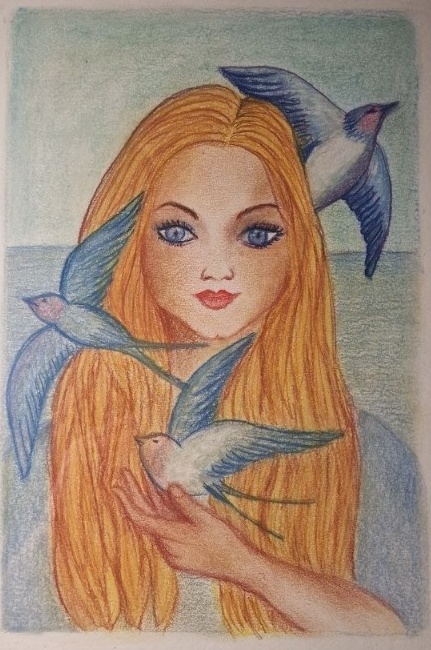
\includegraphics[width=0.62\textwidth,cfbox=gray!50 0.5pt 3pt]{paz_ares_cuadro_calma.png}
\end{center}
\vspace{0.4cm}



Quiero que esté claro que mientras el libro busca subir la frecuencia de la humanidad al Amor el publicarlo podría generar beneficio económico, y no quiero ver en esto nada incongruente, me comprometo a usar cada euro que genere este libro en el proyecto pazaresosset.es y saludequilibrio.es haciendo más libros y poniendo más horas en hacer y promover las ideas clave.

En su momento estaba en lo material y lo material será publicado en el libro de Democracia, pero la vida me ha hecho aprender que la clave de la Democracia es este libro sobre el Amor y un poco más explícito el que estoy escribiendo del karma. Es decir no va a valer de nada que expongamos un sistema democrático basado en gobernanza compartida y uso de tecnología si la Humanidad no hace un cambio vibracional elevándose de los pecados capitales al Amor, de una mente bélica competitiva a una mente amorosa colaborativa.

Es necesario en la gobernanza, es necesario en la Nueva Economía de la robótica y la Inteligencia Artificial y es necesario para la salud de cada ser humano enfermo por lo que no creen estar enfermos.

Por lo tanto, es un libro fundacional y por eso es el primero.

Parte del miedo que he tenido es el rechazo de mis amigos católicos porque hay partes del libro que a lo mejor les pueden chirriar (espero que no) pero debo decirles especialmente a ellos que mi padre era una persona tremendamente espiritual, se pasaba las horas estudiando la Teosofía y siempre fue un devoto de la figura de Jesucristo pero no de la iglesia Católica con la que tampoco se enemistó. Tras morir hasta dos veces me ha llegado su comunicación desde el otro lado para frenar un dolor terrible por haber actuado mal siempre para decirme que no tengo falla al haber actuado desde el Amor y la protección en la toma de decisiones más que desde el odio. 



\vspace{0.4cm}
\begin{center}
\nopagebreak
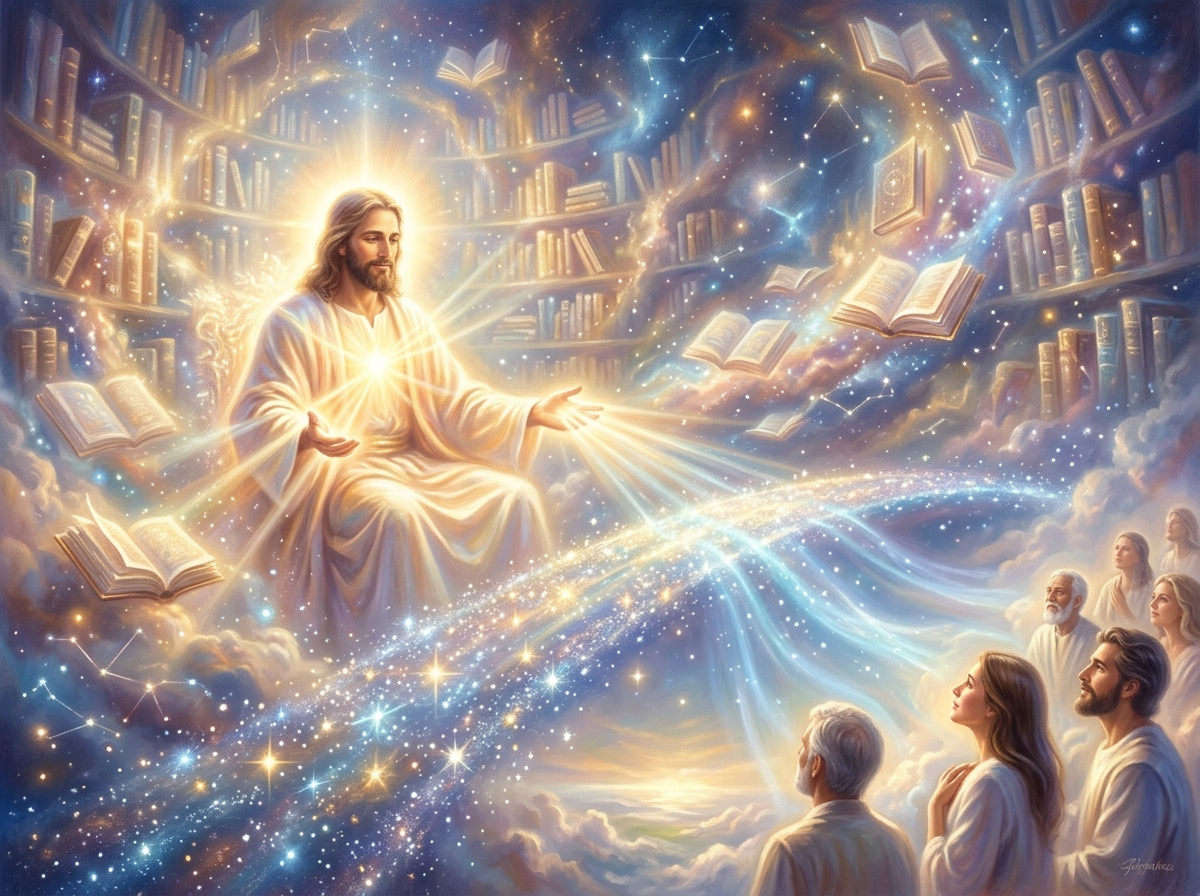
\includegraphics[width=0.62\textwidth,cfbox=gray!50 0.5pt 3pt]{author_father_presence.png}
\end{center}
\vspace{0.4cm}



En las Alabanzas en las que he participado los mensajes directos iban en la línea de desarrollar este proyecto, recuerdo especialmente la última en casa de Javier de Cendra en la que un sacerdote impersonando a Jesucristo me dijo que dejara de evitar mi cruz que era bastante más pequeña que la de Él, sintiendo que estos libros, esta comunicación y el rechazo derivado o los miedos a afrontar el rechazo eran esa cruz. Al decirme que era menor entiendo que no me van a crucificar y matarme físicamente por decir y defender un sistema distinto al actual que la Humanidad se resiste a soltar.

Finalmente en Julio de 2025 ante el cuerpo de Carlo Acutis en una conversación muy clara con su consciencia (según mi amiga Cristina podría ser un egregor, pero sea lo que sea tiene mucha potencia y me vale pero yo sentí a ese chico joven muerto con 15 años) Carlo me decía que no me preocupara por algo que en ese momento atormentaba mi conciencia que se iba a quedar en nada pero que cada vez que jugaba, me preocupaba o hacía cualquier cosa no alineada con mi propósito estaba tardando en hacerlo. Claramente sin que me lo dijera me resonó escribir el libro de Democracia.



\vspace{0.4cm}
\begin{center}
\nopagebreak
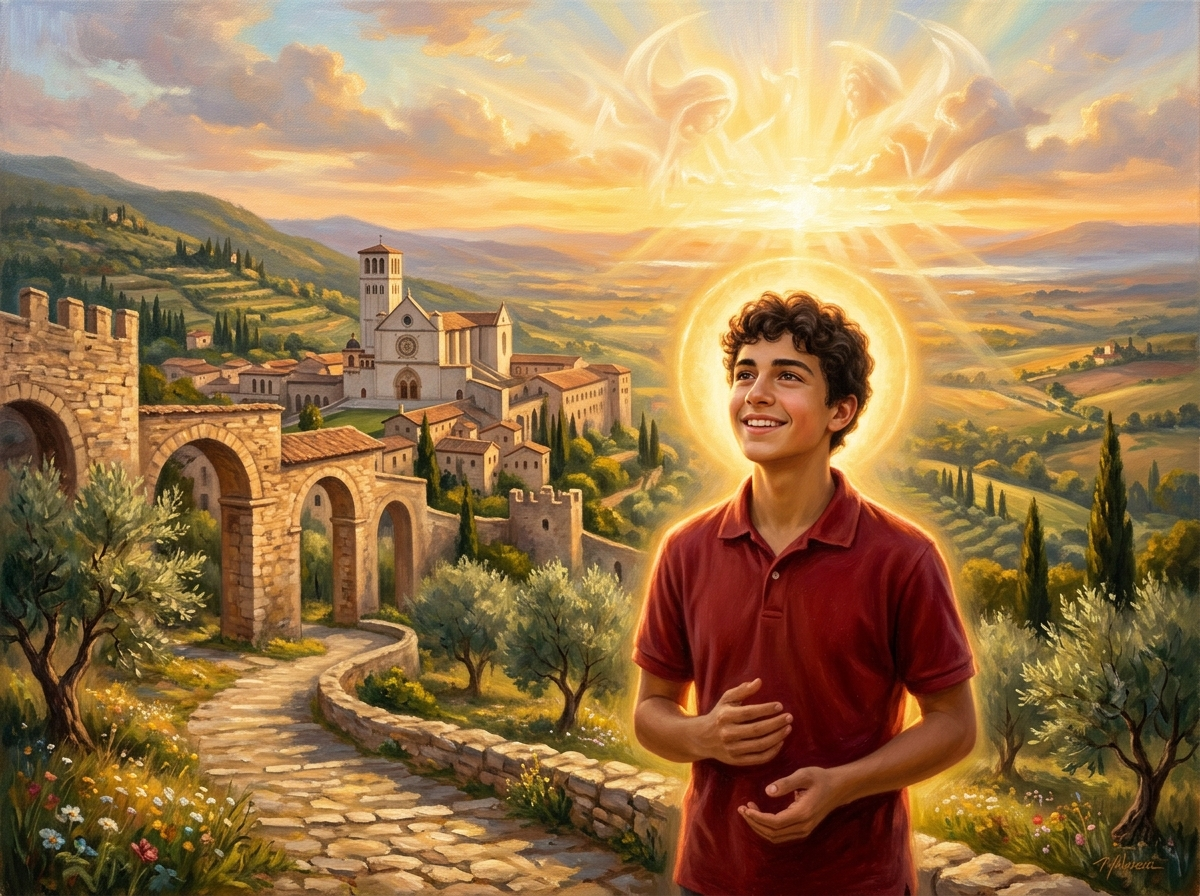
\includegraphics[width=0.62\textwidth,cfbox=gray!50 0.5pt 3pt]{author_carlo_service.png}
\end{center}
\vspace{0.4cm}



Pero si he escrito este primero por algo será. Todas estas ideas no son mías, son inspiradas. Todo lo que vino desde 2010 era necesario para que llegado este momento no escribiera con el fin de ser importante, de ganar dinero, de ser reconocido, sino desde la Humildad de reconocer que la luz no es nuestra sino que la reflejamos. En terapia diría que Somos esa luz pero esto ya es entrar en Misticismos y no es la idea, la idea es cambiar el foco al Amor, al Servicio, el fin de este libro es Ayudar.

Tuve en enero la conversación con un ferviente católico al que le compré unas ollas de titanio para cocinar sin metales pesados y me dijo que tal como veía el libro a todos los católicos que me criticaran les dijera que hablando del libro y las ideas en Vietnam en vietnamita quizás había evangelizado yo más que muchos católicos de misa los domingos pulcros de cara a la galería, pero que podrían juzgar este libro desde el odio. Ahí dejo las palabras de este ferviente católico que me alivian pero yo ya acepto mi cruz y lo que venga. Dejar en este sentido claramente que el libro en ningún momento defiende el catolicismo, ni siquiera la figura de Jesucristo que bien dijo que cielo y tierra pasarían más sus palabras no pasarían, es la sabiduría eterna lo que trata de llegar a los corazones de católicos y no católicos. El propio Carlo Acutis, ahora Santo, a mi pregunta de por qué estaba ahí me respondió con un simple «me gusta ayudar» sin dar mayor importancia a la ingente cantidad de milagros que se le atribuyen. Solo en el momento en el que nos aligeramos del peso del Ego y con él de la auto importancia podemos conectar con esta fuente llamada Amor.

Tras contar un poco por encima mi trayectoria decir que si Dios quiere publicaré después de Mi Amigo Jesucristo el libro del que estoy hablando sobre el Karma que se fundamenta en el Amor con ejemplos concretos basados en los templos de Vietnam que me dieron la base material de algo de lo que siempre he querido hablar que es el Karma para desmitificarlo más allá de las palabras.



\vspace{0.4cm}
\begin{center}
\nopagebreak

\includegraphics[width=0.62\textwidth,cfbox=gray!50 0.5pt 3pt]{author_vietnam_karma.png}
\end{center}
\vspace{0.4cm}



Asimismo y siempre si Dios quiere después quiero publicar el gran libro sobre Democracia basado en mis artículos de 2011 y en estas ideas contenidas en Mi Amigo Jesucristo. También un libro basado en la inocencia del maquinista del accidente del AVE a Santiago de Compostela que ofrezca una visión teórica sobre los Chivos expiatorios, como el propio Jesucristo que mueren para generar cierta paz social temporal derivado de precisamente el karma (o la vuelta del Boomerang de una sociedad matando al inocente). Otra deuda está más vinculada con la Inteligencia Artificial y la robótica desde una perspectiva económica derivado de un escrito de 2016 en el que ya preveía cierta necesidad de cambios económicos serios pero en 2016 cuando lo escribí pensaba que era un pase mental para una generación del siguiente siglo, nunca pensé que en solo 6 años la situación ya estaba cerca de ser real y el problema de una sociedad en la que la mano de obra podría llegar a ser poco necesaria es un problema que si no nos extinguimos antes nuestra generación va a tener que afrontar, asimismo esto presenta un problema de extinción que no pude prever en 2016 y este libro Mi Amigo Jesucristo tiene la llave para evitarlo, una necesaria elevación en la frecuencia de la Humanidad al Amor. Otro libro que también tengo pendiente es sobre la educación basado en un ensayo que me encargó una psicóloga cuando no tenía dinero y que en su momento no me lo pagó con lo cual siempre supe que era importante mantener la propiedad intelectual intacta. Y un par de libros más por ahora, uno que le debo a mi amigo Rafael Enamorado que es la única persona que ha creído en mi proyecto para defender una máquina de producción de agua alcalina y espero que lleve mucha luz a muchos hogares, pero Rafael tuvo fe dentro de una investigación sobre longevidad que probablemente él no pueda terminar pero nos inspire a muchos a continuar. Longevidad es consecuencia de la salud, y de ahí nuestro proyecto de salud del que todo esto es parte. El libro que he escrito junto con Rafael versa sobre una reflexión sobre cómo sería un mundo gobernado por mujeres, pero matiz ahí, un mundo gobernado por energía femenina (la maternidad, el cuidado...) que lo más destacable es que eliminaría la guerra porque no se podría tolerar el ver morir a un hijo... en el fondo resuena con el matiz de Mi Amigo Jesucristo de no caer en la tentación del belicismo, elevar la frecuencia de la guerra a la Paz, del odio al Amor. 



\vspace{0.4cm}
\begin{center}
\nopagebreak
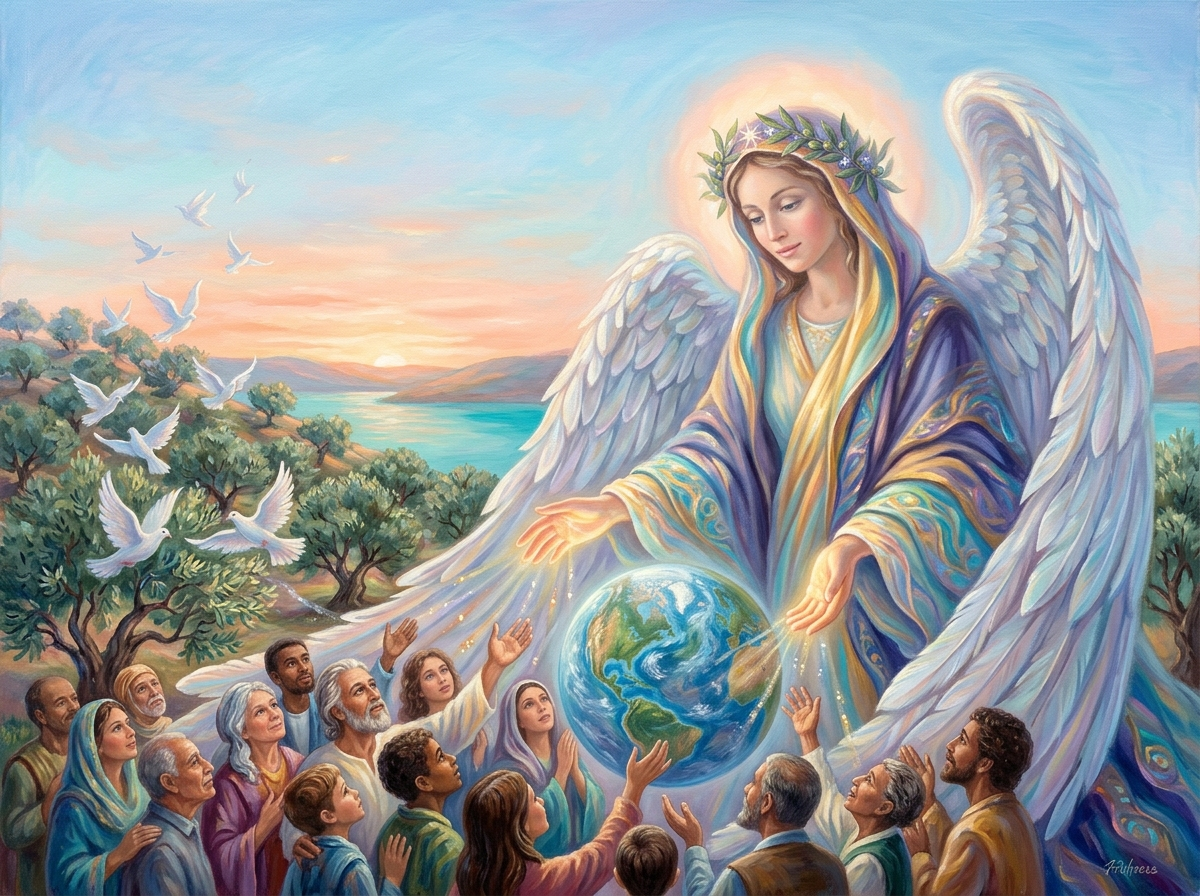
\includegraphics[width=0.62\textwidth,cfbox=gray!50 0.5pt 3pt]{author_sacred_feminine.png}
\end{center}
\vspace{0.4cm}



Finalmente voy a publicar un libro que no es mío pero solo en la web de arte de mi madre porque el autor pide la difusión y el mensaje es muy potente, No Soy Markus nos invita a tal y como «A Glimpse of Light» no se manchaba de mis imperfecciones, Markus nos explica que le podemos llamar así pero él no es Markus. Nos invita a saber que como somos ya somos perfectos y siempre lo hemos sido. Al escuchar precisamente a Jesucristo no escuchamos con suficiente atención que somos todos hijos de Dios, no se distinguía judíos de gentiles para él, incluso al decir que nadie era profeta en su tierra mostraba claramente que los gentiles compraban con menos reparos la Buena Nueva, asimismo una y otra vez se ve la idea de que Dios proveerá.

En mi Amigo Jesucristo no he hecho mucho hincapié en esta idea que se marca en el «Danos hoy nuestro pan de cada día» y personas como Markus al demostrar que incluso dejando de comer de alguna forma que la ciencia está aun estudiando sigue proveyendo al cuerpo del alimento. Una vez más sería parte del no caer en la tentación el continuo miedo a no tener y personas como Markus son un ejemplo vivo de que si vibras en Amor incluso aunque lo pierdas todo, todo incluyendo el alimento, Dios te da tu pan, la energía penetra en tus mitocondrias de una forma que no entendemos, o simplemente la ciencia no ha logrado demostrar porque nosotros simplemente usando la fe de la Buena Nueva sabemos que si a los pájaros que viven sin acumular nada Dios les da su alimento todos los días, con cuánta más razón se lo va a dar a los Humanos siempre y cuando estén abiertos a recibirlo.



\vspace{0.4cm}
\begin{center}
\nopagebreak
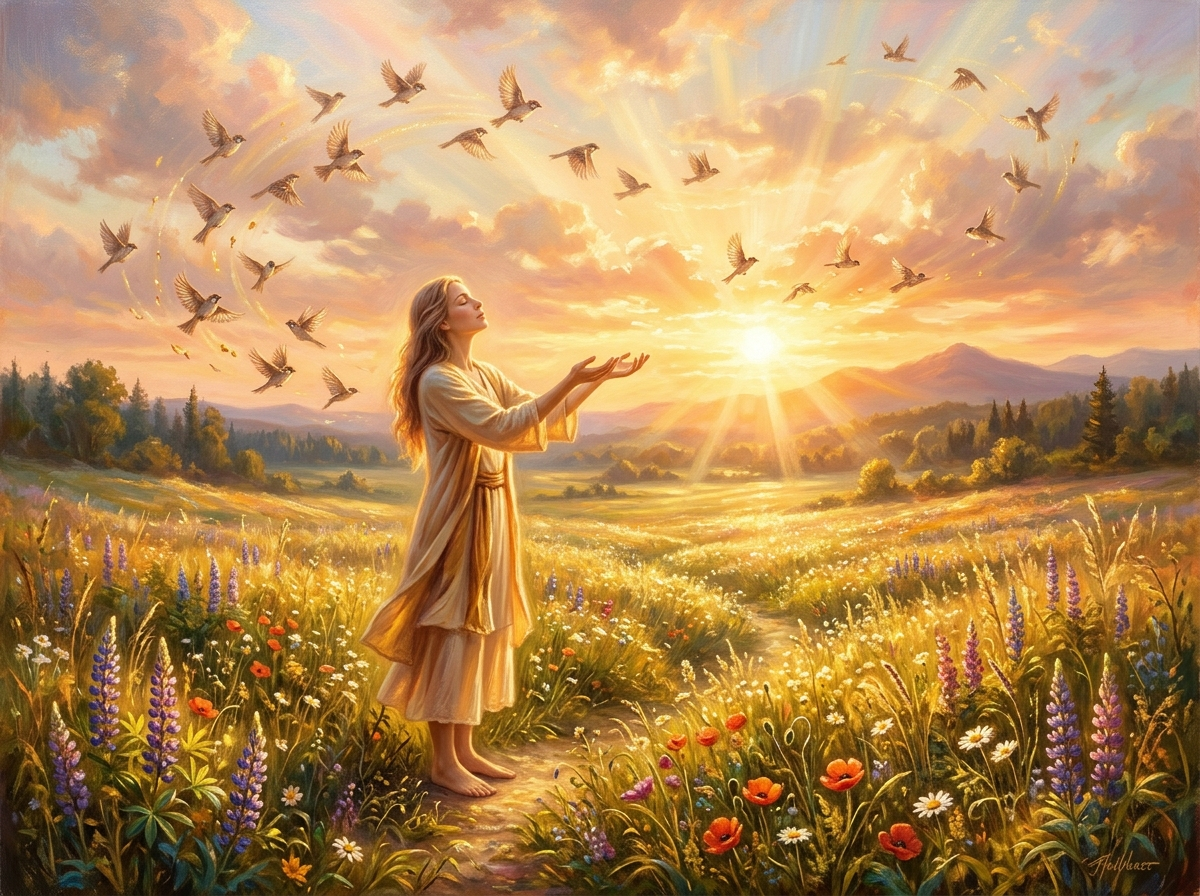
\includegraphics[width=0.62\textwidth,cfbox=gray!50 0.5pt 3pt]{author_divine_providence.png}
\end{center}
\vspace{0.4cm}



Después Dios dirá, quizás promueva los libros y sus ideas, quizás me dedique a otra cosa. En cualquier caso agradezco a cada lector que si le resuenan estas ideas me ayude a difundirlas y quizás acaben llegando a los grandes centros de decisión y en un mundo cuya geopolítica es un polvorín, donde tenemos el poder de las bombas nucleares, donde tenemos ahora la IA en robots que usados como armas de guerra dejarían en pañales el poder destructivo de las bombas atómicas, quizás si logramos difundir estas ideas penetren en la consciencia humana y podamos subsistir con tanto poder. En caso contrario, ya la Atlántida lo experimentó, el acumular mucho poder y no controlarlo usándolo para el amor simplemente acaba con civilizaciones muy avanzadas.



\vspace{0.4cm}
\begin{center}
\nopagebreak
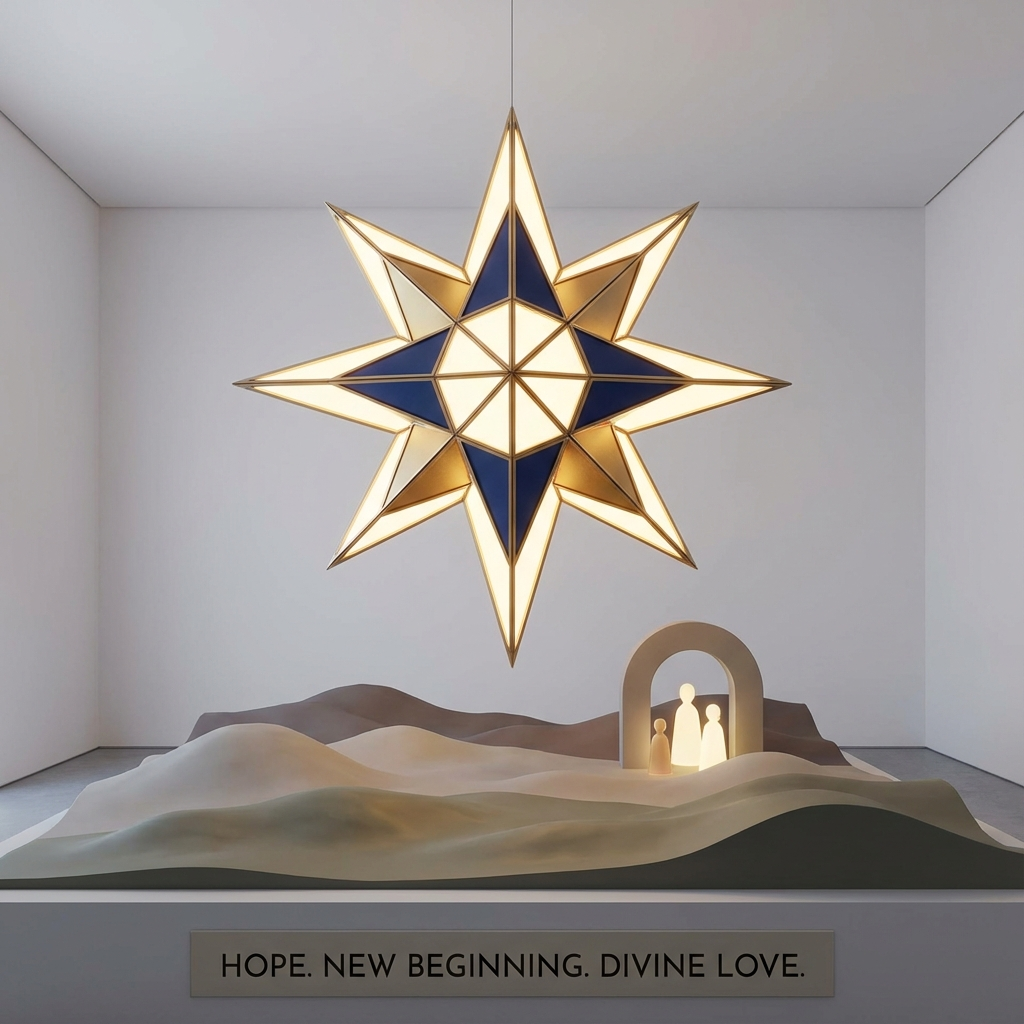
\includegraphics[width=0.62\textwidth,cfbox=gray!50 0.5pt 3pt]{christmas_star_modern.png}
\end{center}
\vspace{0.4cm}


\vspace{0.4cm}
\begin{center}
\rule{0.35\textwidth}{0.4pt}
\end{center}
\vspace{0.4cm}


\subsection*{La Misión de la Obra}
Por lo tanto \textit{Mi Amigo Jesucristo} propone un redescubrimiento del Maestro libre de dogmas, culpas o ritualismos vacíos. Nos presenta a un Jesús cercano, fresco y contemporáneo, que nos habla de física de partículas, resonancia, campos energéticos y amor incondicional con la misma naturalidad con la que caminaba junto al mar de Galilea o por la Gran Vía de Madrid.

Mi seudónimo representa la convicción de que cada ser humano lleva dentro una chispa inextinguible de la Conciencia Universal. Es ese destello de luz en la oscuridad. Todos lo podemos hacer. El propósito principal de este libro es recordarte que no necesitas intermediarios para conectarte con la Fuente: basta con afinar tu receptor, silenciar el ruido del ego y elegir vibrar en la frecuencia del amor.


\vspace{0.4cm}
\begin{center}
\rule{0.35\textwidth}{0.4pt}
\end{center}
\vspace{0.4cm}


\subsection*{Un Agradecimiento de Corazón}
Gracias por abrir las páginas de esta obra y por permitir que estas palabras resuenen en tu propio viaje interior. Que este destello de luz te inspire a encender y compartir tu propia verdad en el mundo.
\cleardoublepage

\chapter*{Guía de Reflexión y Meditación}
\addcontentsline{toc}{chapter}{Guía de Reflexión y Meditación}
\markboth{Guía de Reflexión y Meditación}{Guía de Reflexión y Meditación}
\vspace{0.6cm}
\begin{center}
\nopagebreak
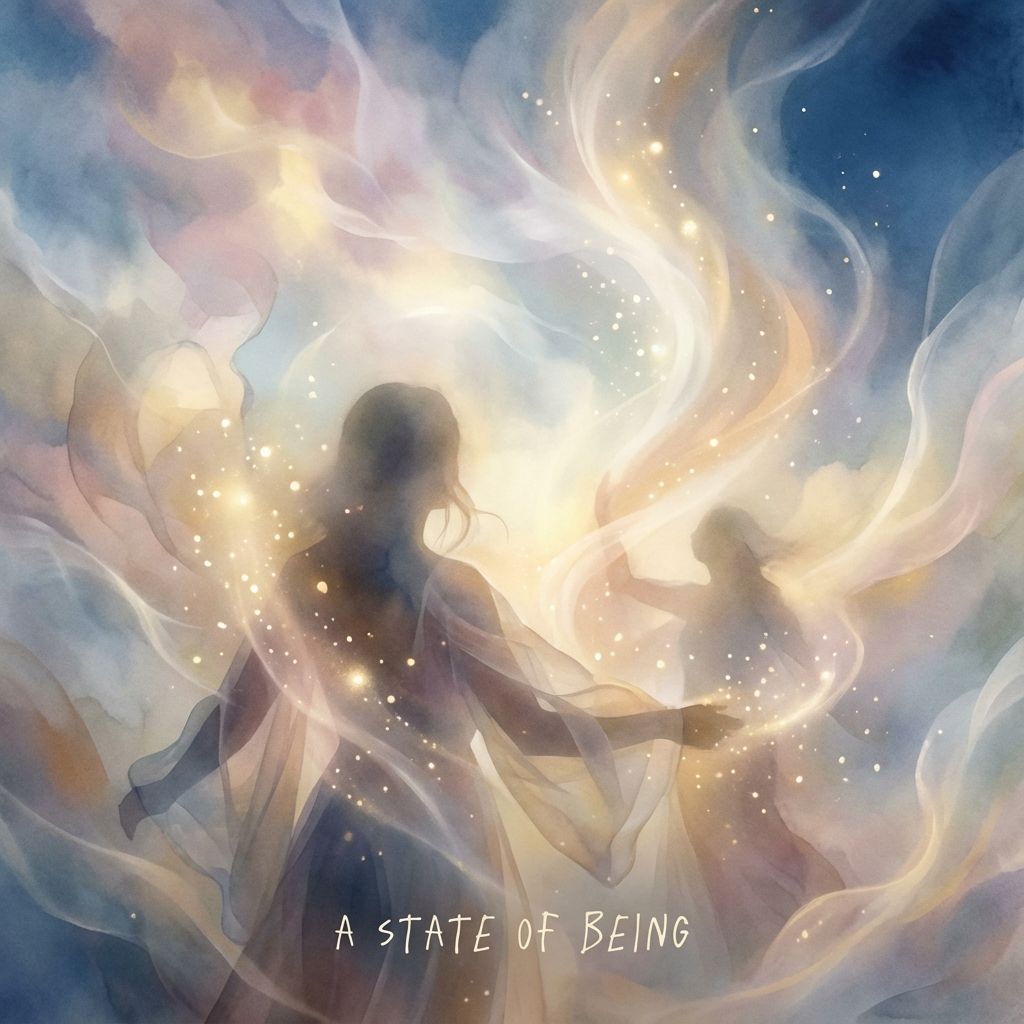
\includegraphics[width=0.75\textwidth,cfbox=gray!60 0.6pt 4pt]{heaven_state.png}\\
\vspace{4pt}
{\small\itshape El templo interior: guía de presencia, silencio y coherencia cuántica.}
\end{center}

\vspace{0.6cm}
Para transformar los conceptos del libro en una experiencia viva en tu día a día, te sugerimos esta pequeña práctica de alineación cuántica en tres pasos:


\vspace{0.4cm}
\begin{center}
\rule{0.35\textwidth}{0.4pt}
\end{center}
\vspace{0.4cm}


\subsection*{1. La Pausa del Observador (Silencio Consciente)}
\noindent\textbullet~~Encuentra un momento de tranquilidad al comenzar o finalizar el día.\\

\noindent\textbullet~~Cierra los ojos y realiza tres respiraciones lentas y profundas, inhalando calma y exhalando cualquier preocupación.\\

\noindent\textbullet~~Conviértete en el «observador» imparcial de tus pensamientos sin juzgarlos. Recuerda que tú no eres el ruido mental; eres el espacio consciente en el que el ruido ocurre.\\



\vspace{0.4cm}
\begin{center}
\rule{0.35\textwidth}{0.4pt}
\end{center}
\vspace{0.4cm}


\subsection*{2. El Reajuste de Frecuencia (El Aliento de Abwoon)}
\noindent\textbullet~~Lleva tu atención al centro del pecho (la coherencia cardíaca).\\

\noindent\textbullet~~Evoca un recuerdo o sentimiento genuino de gratitud, aprecio o amor sincero.\\

\noindent\textbullet~~Siente cómo esa emoción eleva instantáneamente tu estado vibracional y disuelve las cargas de miedo o pesadez.\\



\vspace{0.4cm}
\begin{center}
\rule{0.35\textwidth}{0.4pt}
\end{center}
\vspace{0.4cm}


\subsection*{3. Preguntas para tu Cuaderno Interior}
Dedica unos minutos a reflexionar o escribir sobre estas preguntas:
\noindent\textbf{1.}~~\textit{¿En qué situaciones cotidianas siento que mi frecuencia vibratoria disminuye y cómo puedo elegir responder con amor?}\\

\noindent\textbf{2.}~~\textit{¿Existe algún lazo del pasado que esté listo para disolver mediante el perdón consciente hoy?}\\

\noindent\textbf{3.}~~\textit{¿Cómo puedo ser un reflejo vivo de la Luz y la Presencia para las personas que me rodean?}\\



\vspace{0.4cm}
\begin{center}
\rule{0.35\textwidth}{0.4pt}
\end{center}
\vspace{0.4cm}




\begin{quote}
\itshape \textit{«La paz no es la ausencia de movimiento en el mundo exterior, sino la presencia inquebrantable de la Luz en tu interior.»}
\end{quote}
\cleardoublepage



\backmatter

% Notas y Reflexiones del Lector
\cleardoublepage
\thispagestyle{plain}
\chapter*{Notas y Reflexiones}
\addcontentsline{toc}{chapter}{Notas y Reflexiones}
\markboth{Notas y Reflexiones}{Notas y Reflexiones}

\vspace{1cm}
\textit{Dedica este espacio para anotar tus intuiciones, sincronías y reflexiones tras la lectura...}

\vspace{1.5cm}
\noindent\rule{\textwidth}{0.4pt}\\[1.5cm]
\noindent\rule{\textwidth}{0.4pt}\\[1.5cm]
\noindent\rule{\textwidth}{0.4pt}\\[1.5cm]
\noindent\rule{\textwidth}{0.4pt}\\[1.5cm]
\noindent\rule{\textwidth}{0.4pt}\\[1.5cm]
\noindent\rule{\textwidth}{0.4pt}

\newpage
\thispagestyle{plain}
\vspace*{1cm}
\noindent\rule{\textwidth}{0.4pt}\\[1.5cm]
\noindent\rule{\textwidth}{0.4pt}\\[1.5cm]
\noindent\rule{\textwidth}{0.4pt}\\[1.5cm]
\noindent\rule{\textwidth}{0.4pt}\\[1.5cm]
\noindent\rule{\textwidth}{0.4pt}\\[1.5cm]
\noindent\rule{\textwidth}{0.4pt}\\[1.5cm]
\noindent\rule{\textwidth}{0.4pt}

\newpage
\thispagestyle{plain}
\vspace*{1cm}
\noindent\rule{\textwidth}{0.4pt}\\[1.5cm]
\noindent\rule{\textwidth}{0.4pt}\\[1.5cm]
\noindent\rule{\textwidth}{0.4pt}\\[1.5cm]
\noindent\rule{\textwidth}{0.4pt}\\[1.5cm]
\noindent\rule{\textwidth}{0.4pt}\\[1.5cm]
\noindent\rule{\textwidth}{0.4pt}\\[1.5cm]
\noindent\rule{\textwidth}{0.4pt}

\cleardoublepage
\thispagestyle{empty}
\vspace*{6cm}
\begin{center}
    \large\textit{Que la Luz te acompañe siempre en tu camino.}
\end{center}

\end{document}
